\documentclass{beamer}
\usepackage{beamerthemeshadow}
\usepackage[ngerman]{babel}
\usepackage[utf8]{inputenc}
%Tabellen:
	\usepackage{slashbox} %schrägstich in tabelle möglich
	\usepackage{multirow}
%Mathematik:
	\usepackage{dsfont} %Symbole
	\usepackage{amsmath} %Umgebung
	\usepackage{amssymb} %Symbole
	\usepackage{bbm} %doppelstreifen bei buchstaben (zb symbol für ganze zahlen \mathbbm{Z})
%Grafiken:
	\usepackage{graphics}
	\usepackage{graphicx}
	\usepackage{picinpar} %bilder so einfügen, dass text um bilder weiterläuft
	\usepackage{float} %\begin{figure}[H] => Grafik wird HIER eingefügt!
%Pseudo Code:
	\usepackage{algorithmic}
	\usepackage{algorithm}
	
\DeclareMathOperator*{\argmin}{arg\,min}

\beamersetuncovermixins{\opaqueness<1>{25}}{\opaqueness<2->{15}}
\setbeamertemplate{footline} %seitenzahl rechts unten
{%
  \leavevmode%
 \begin{beamercolorbox}%
    [wd=.5\paperwidth,ht=2.5ex,dp=1.125ex,leftskip=.3cm,rightskip=.3cm]%
    {author in head/foot}%
    \usebeamerfont{author in head/foot}%
    \hfill\insertshortauthor
  \end{beamercolorbox}%
  \begin{beamercolorbox}%
    [wd=.5\paperwidth,ht=2.5ex,dp=1.125ex,leftskip=.3cm ,rightskip=.3cm]%
    {title in head/foot}%
    \usebeamerfont{title in head/foot}%
    \insertshorttitle\hfill\insertframenumber{}/\inserttotalframenumber
  \end{beamercolorbox}%
}%

\beamertemplatenavigationsymbolsempty % Abschalten der kleinen Navigationsleiste am unteren Rand

\begin{document}
\title{Online-Marketing der Interhyp AG}
\subtitle{Analyse von Tracking-Daten} 
\author[D. Fuckner \& M. Vogler]{Daniel Fuckner\\Markus Vogler\\Betreuer: Fabian Scheipl}
\institute{Statistisches Consulting\\Institut für Statistik\\Ludwig-Maximilians-Universität München}
\date{12.08.2014} 

\begin{frame}
	\titlepage
\end{frame}

\begin{frame}\frametitle{Inhaltsverzeichnis}
	\tableofcontents[hideallsubsections]
\end{frame}

\section{Einleitung} 

\begin{frame}\frametitle{Einleitung} 
	\begin{itemize}
		\item Interhyp AG ist Vermittler für private Baufinanzierungen
		\item Primäres Ziel des Marketing ist die Kundenakquise
		\item Etwa $80 \%$ aller Kundenanträge werden online abgeschickt
		\item Online-Marketing verfügt über verschiedene Kanäle
		\item Refined Labs GmbH ist verantwortlich für das Online-Tracking der Werbekampagnen der Interhyp AG
	\end{itemize}
\end{frame}

\begin{frame}\frametitle{Entstehung eines Funnels (Quelle: Interhyp AG)}
	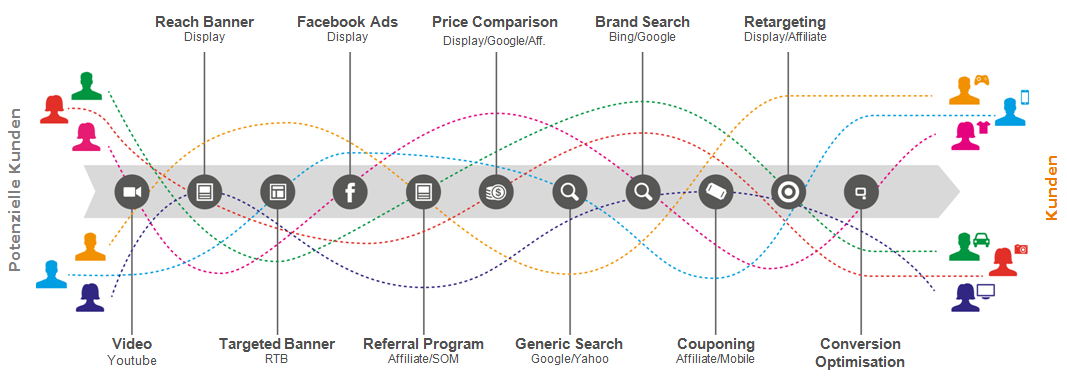
\includegraphics[scale=0.38]{customerJourney.png}\\
	\centering Unterschiede zwischen konvertierten und nicht-konvertierten Funnels?
\end{frame}
\section{Deskriptive Analyse}

\begin{frame}\frametitle{Inhalt}
	\tableofcontents[currentsection,hideallsubsections]
\end{frame}

\begin{frame}\frametitle{Beispiel für einen Auszug aus der Datenbank}
	\begin{table}[H]
		\begin{center}
			\begin{tabular}{|c|l|c|c|c|c|}
				\hline
				ID & Campaign 									 & Transaction & Position & ... \\ \hline\hline
				1  & Affiliate - Partnerprogramm & 0					 & 1		    & ... \\ \hline
				1  & SEM - Brand                 & 0					 & 2		    & ... \\ \hline
				1  & Direct                      & 0					 & 3		    & ... \\ \hline
				1  & Direct                      & 1					 & 4		    & ... \\ \hline
				2  & Display                     & 0					 & 1		    & ... \\ \hline
				2  & SEM - Generisch             & 0					 & 2		    & ... \\ \hline
				2  & Social Media                & 0					 & 3		    & ... \\ \hline
			\end{tabular} 
		\end{center}
	\end{table}
\end{frame}

\begin{frame}\frametitle{Datenlage} 
	\begin{itemize}
		\item SQL-Dump mit Größe von circa $13$ Gigabyte
		\item Einteilung in konvertierte und nicht-konvertierte Funnels
		\item Kampagnen in Form einer Baumstruktur organisiert
		\item Festlegung auf $17$ Kategorien
		\item \textit{Views} liegen in den nicht-konvertierten Funnels nur vor, wenn diese bei einem anderen Kunden der Refined Labs GmbH konvertiert sind
		\item $ 297,963 $ \textit{Clicks} für die konvertierten und $ 9,550,802 $ \textit{Clicks} für die nicht-konvertierten Funnels
		\item Erstellung von Features
	\end{itemize}
\end{frame}

\subsection{Views in den konvertierten Funnels}

\begin{frame}\frametitle{clickCount}
	\begin{columns}
		\column{7cm}
			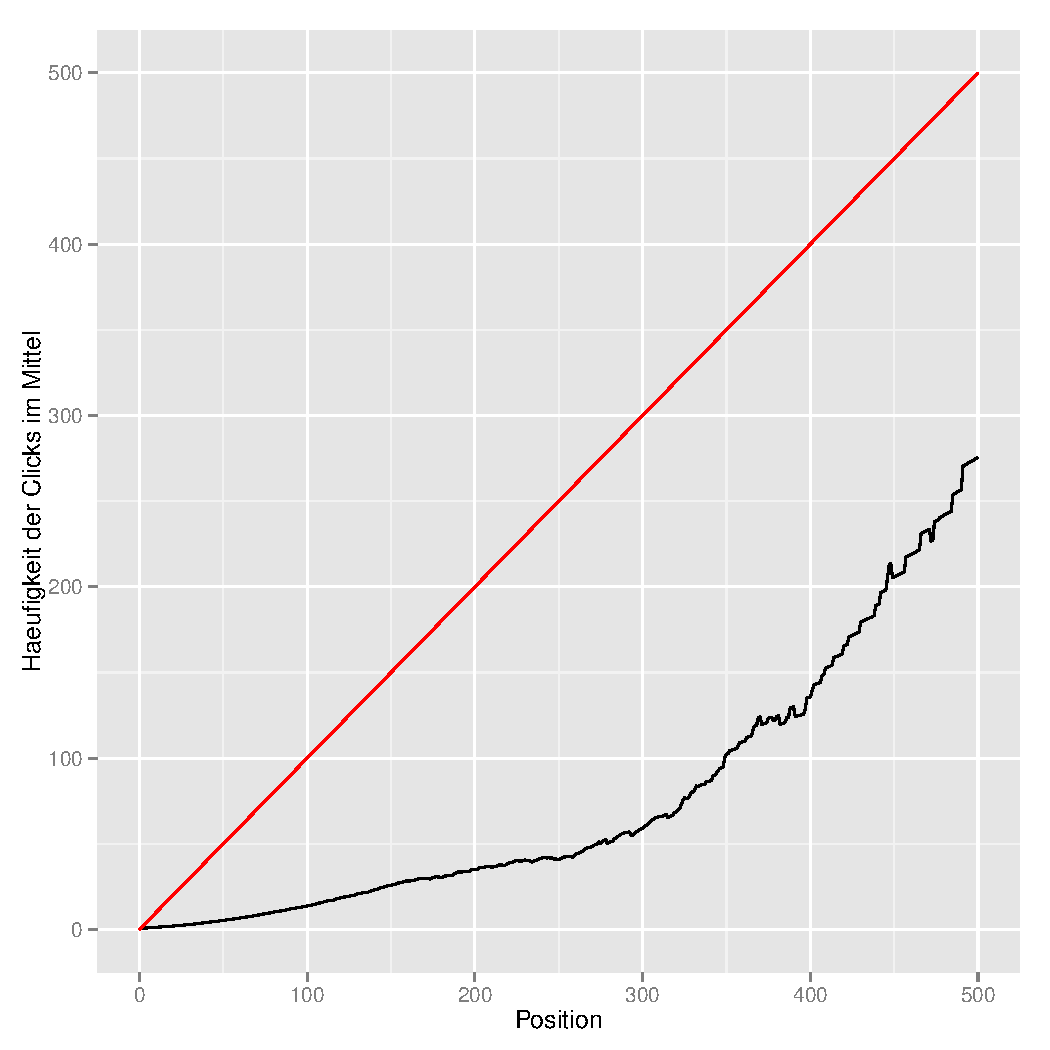
\includegraphics[scale=0.39]{clickCountSucc.pdf}
		\column{4cm}
			\begin{itemize}
				\item Anzahl der Clicks bis zur aktuellen Position
				\item Gemittelt über alle konvertierten Funnels
				\item Mehr \textit{Views} als \textit{Clicks}
			\end{itemize}
	\end{columns}
\end{frame}

%\begin{frame}\frametitle{hasClicked}
	    %\centering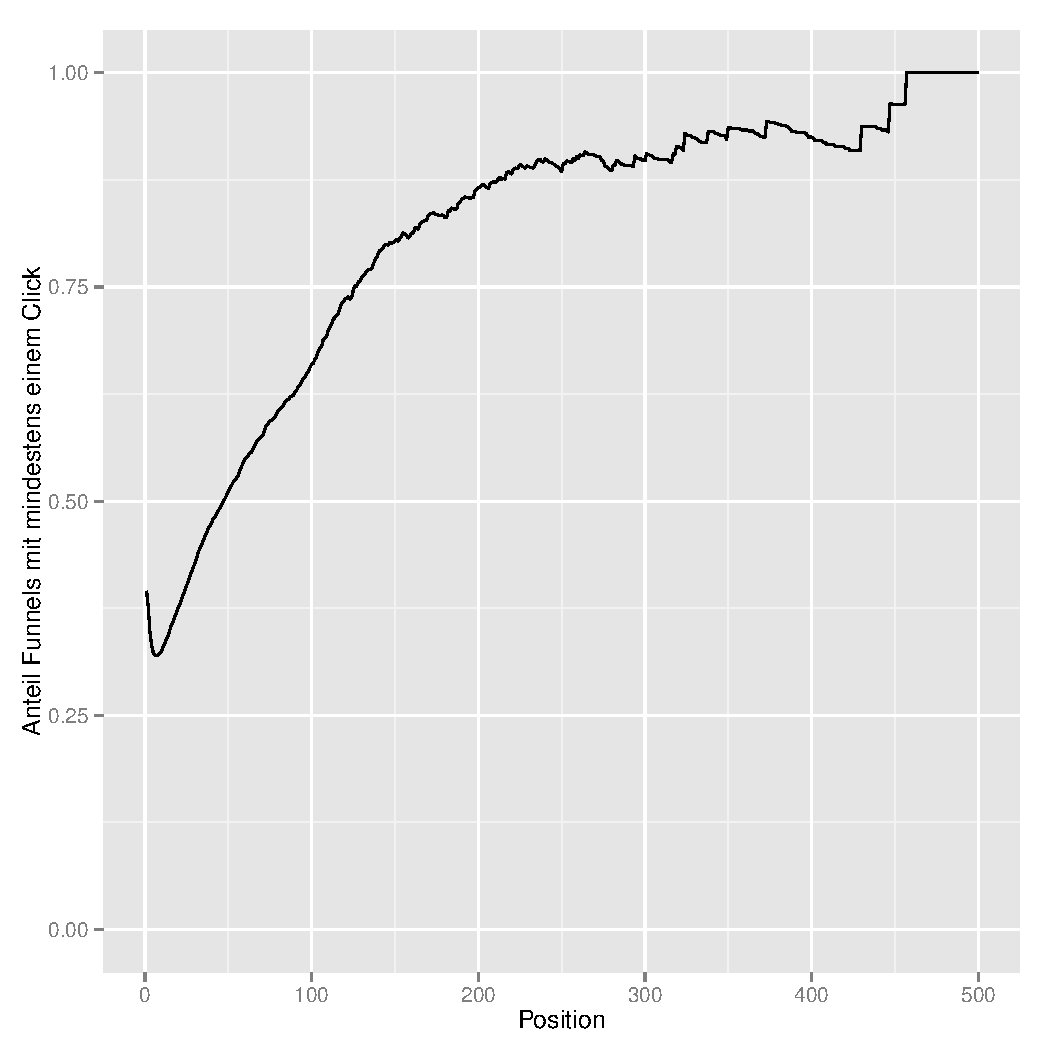
\includegraphics[scale=0.39]{hasClickedSucc.pdf}
%\end{frame}

\begin{frame}\frametitle{Beschreibung der Kampagnen}
	\begin{table}[H]
		\tiny
		\begin{center}
			\begin{tabular}{|l|p{7cm}|}
				\hline \textbf{Kampagne} & \textbf{Beschreibung}\\ \hline
				\hline Affiliate - Partnerprogramm & Partner, die Werbemittel einbinden\\
				\hline Affiliate - Rest & Partner, die Zinsvergleich bereitstellen\\ 
				\hline Direct & Direkte Eingabe von \textit{www.interhyp.de}\\ 
				\hline Display & Bannerschaltungen\\
				\hline E-Mailing & Mails an Interessenten, die schon einen Antrag o.ä. gestellt haben\\
				\hline Generic & Unbezahlter Link\\
				\hline Kooperationen - Focus & \multirow{5}{7cm}{Individuelle Zusammenarbeit mit größeren Partnern}\\
				Kooperationen - Immonet & \\
				Kooperationen - Immoscout24 & \\
				Kooperationen - Immowelt & \\
				Kooperationen - Rest & \\
				\hline Newsletter & Regelmäßige Rundschreiben\\
				\hline SEM - Brand & \multirow{3}{7cm}{Bezahlte Suchergebnisse}\\
				SEM - Remarketing & \\
				SEM - Generisch & \\
				\hline SEO & Unbezahlte Suchergebnisse\\
				\hline Social Media & \textit{facebook} und \textit{gutefrage.net}\\
				\hline
			\end{tabular} 
		\end{center}
	\end{table}
\end{frame}

\begin{frame}\frametitle{campaign}
	\begin{columns}
		\column{7cm}
			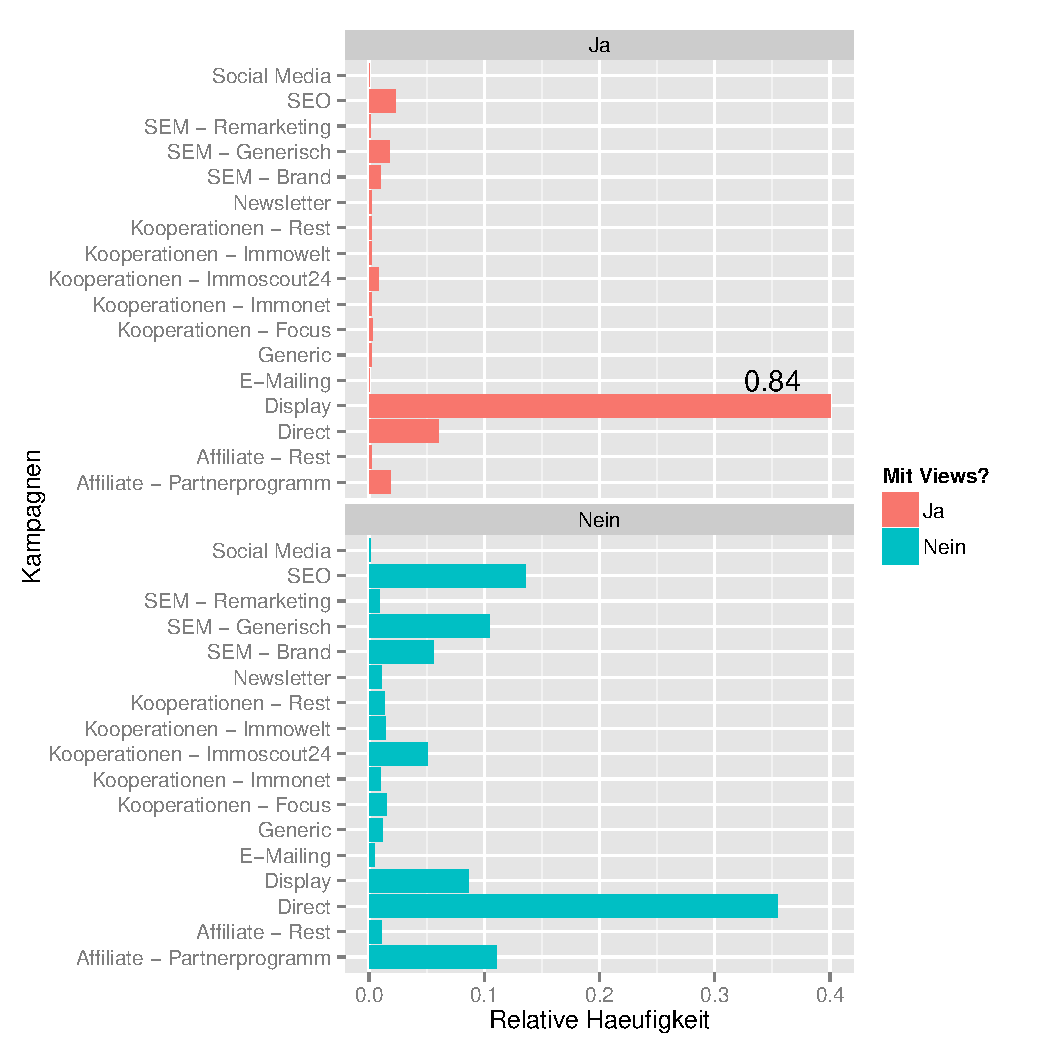
\includegraphics[scale=0.39]{campaignSucc.pdf}
		\column{4cm}
			\begin{itemize}
				\item Hauptsächlich \textit{Display} bei Berücksichtigung der \textit{Views}
				\item Ausgewogenere Verteilung wenn \textit{Views} gelöscht werden
			\end{itemize}
	\end{columns}
\end{frame}

\subsection{Vergleich von konvertierten und nicht-konvertierten Funnels}

%\begin{frame}\frametitle{weekday}
	    %\centering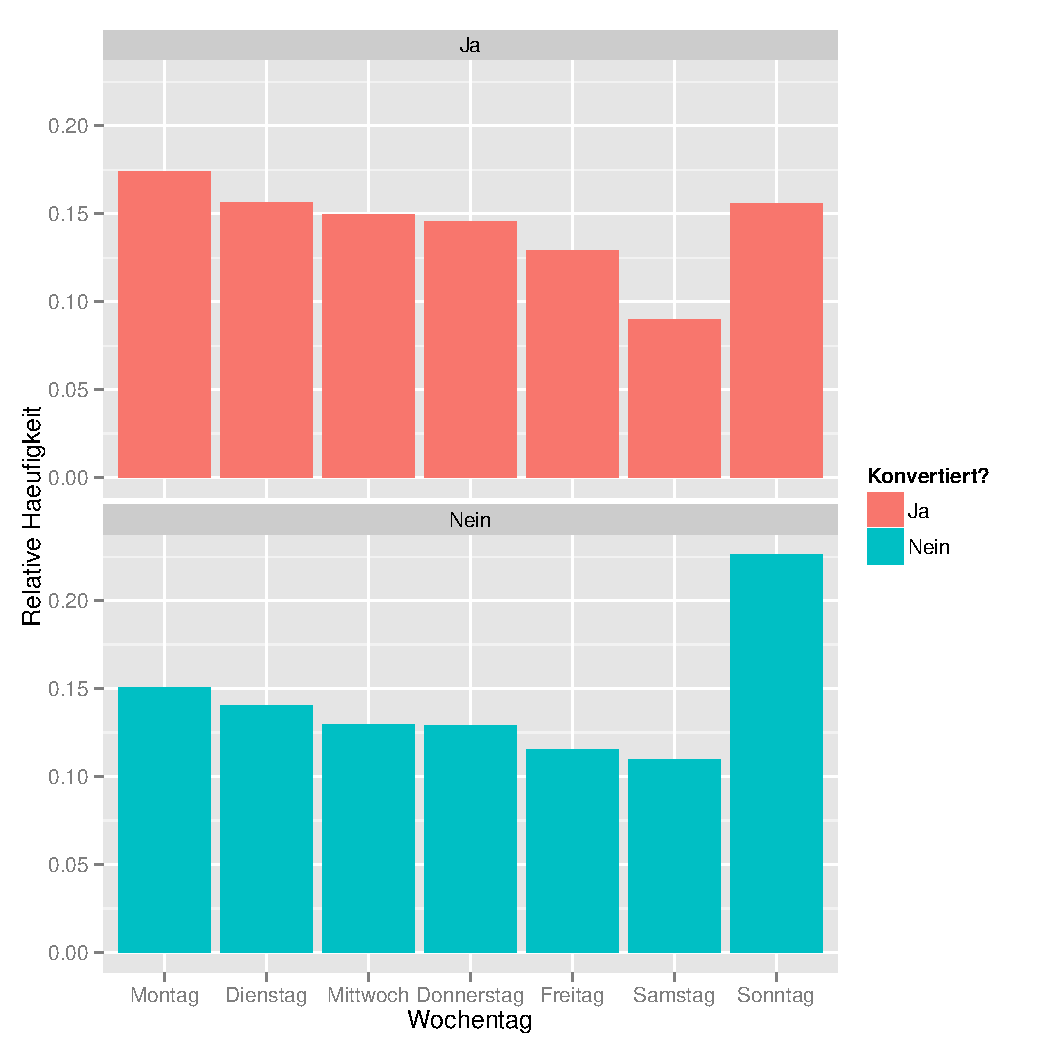
\includegraphics[scale=0.3]{weekday.pdf}
%\end{frame}

%\begin{frame}\frametitle{hour}
	    %\centering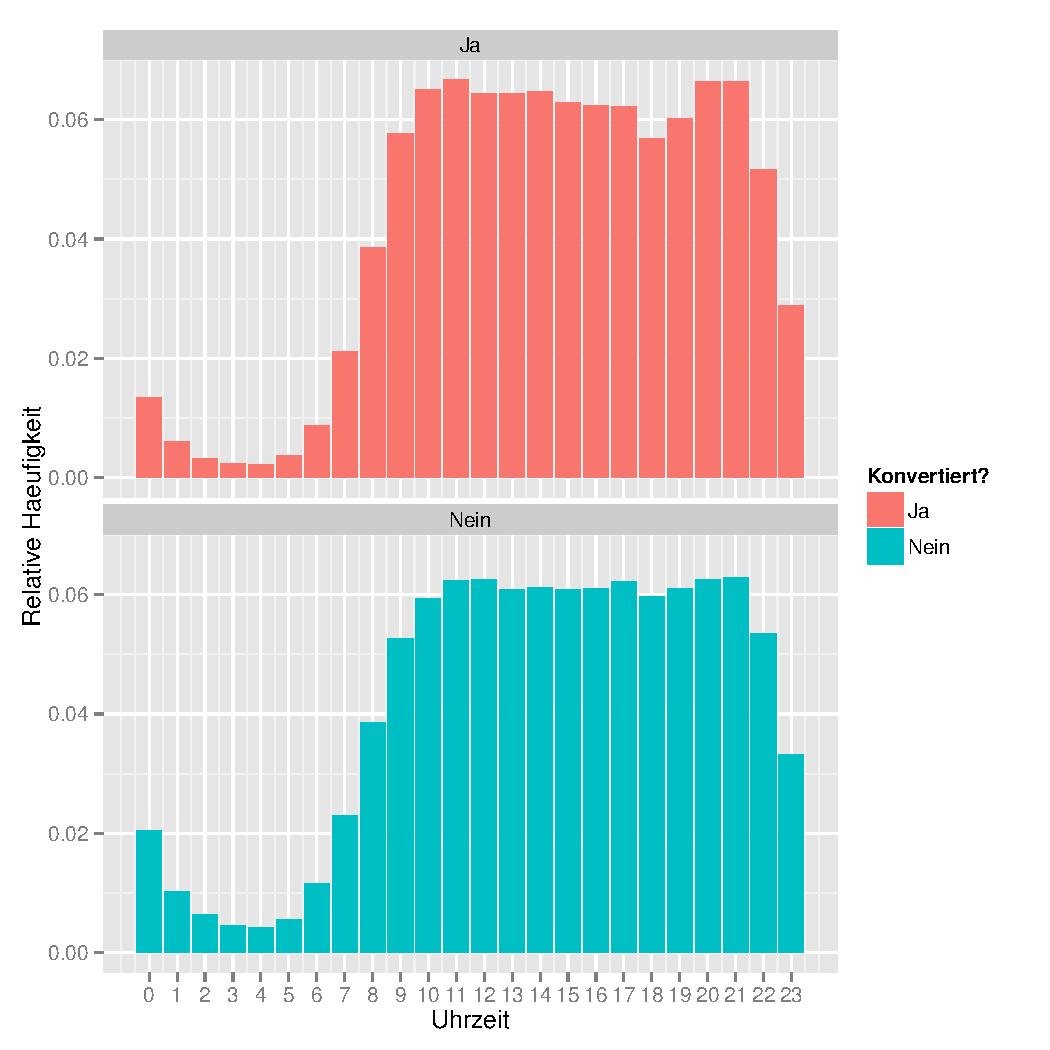
\includegraphics[scale=0.3]{hour.pdf}
%\end{frame}

\begin{frame}\frametitle{campaign}
	\begin{columns}
		\column{7cm}
			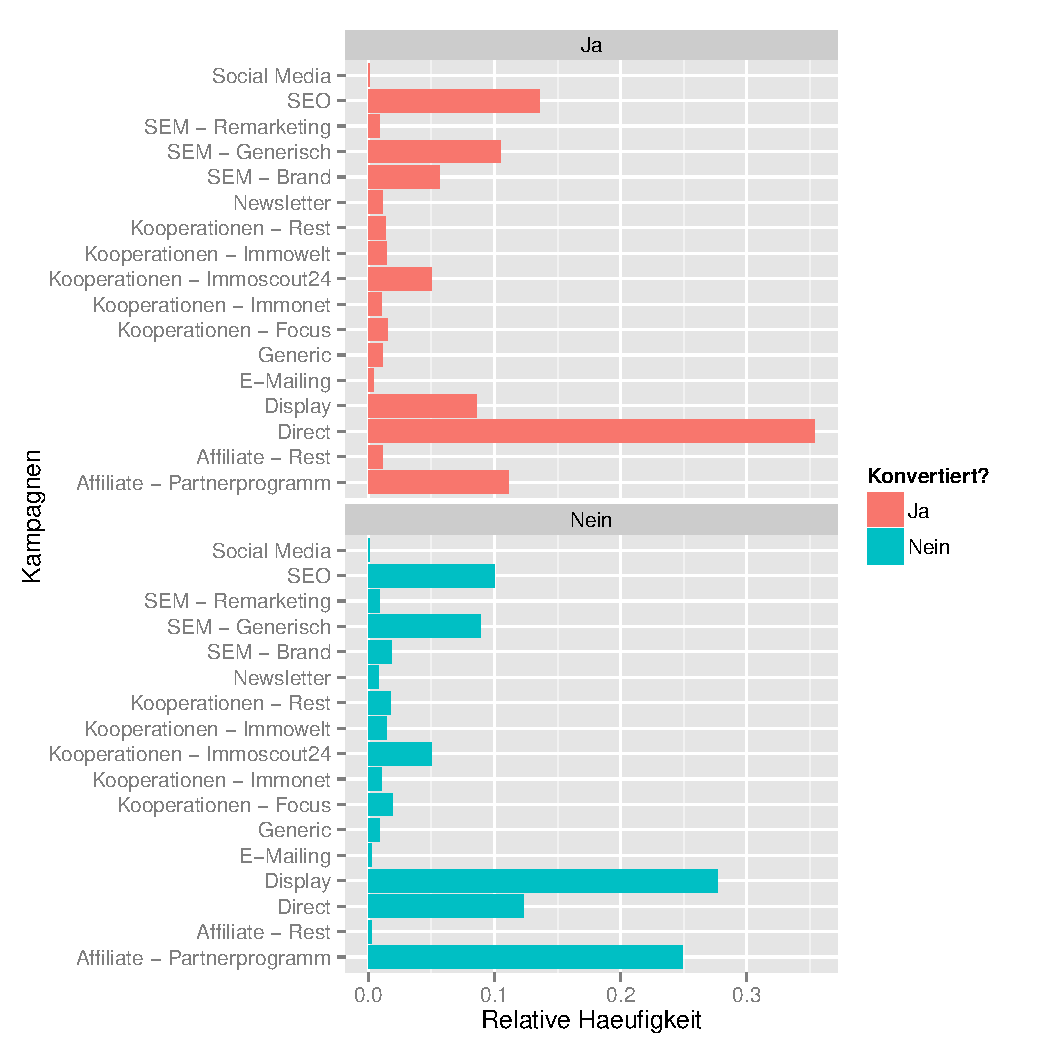
\includegraphics[scale=0.39]{campaign.pdf}
		\column{4cm}
			\begin{itemize}
				\item \textit{Direct} am häufigsten in den konvertierten Funnels
				\item \textit{Display} und \textit{Affiliate - Partnerprogramm} am häufigsten in den nicht-konvertierten Funnels
			\end{itemize}
	\end{columns}
\end{frame}

\begin{frame}\frametitle{funnelLength}
	\begin{columns}
		\column{7cm}
			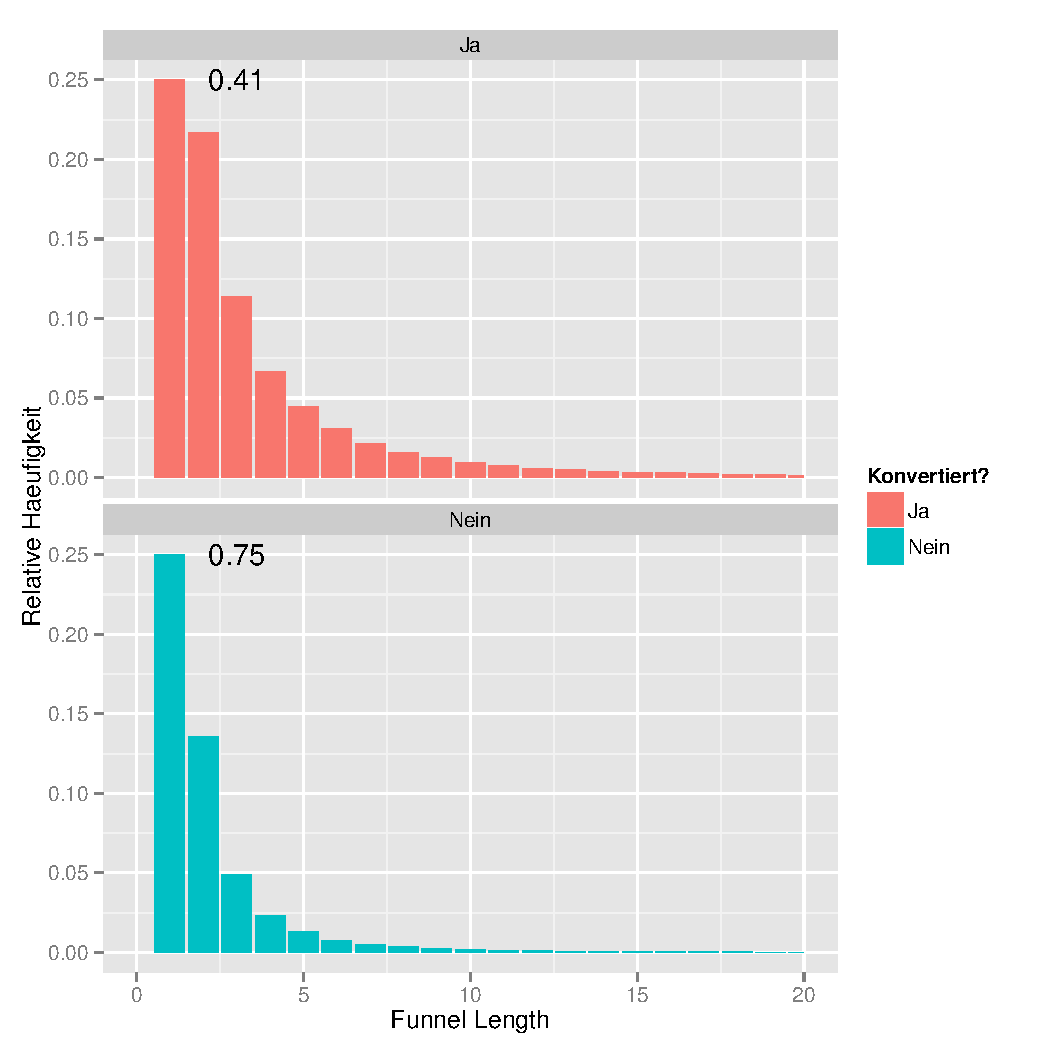
\includegraphics[scale=0.39]{funnelLength_First.pdf}
		\column{4cm}
			\begin{itemize}
				\item Anzahl Kontaktpunkte eines Funnels
				\item Kurze Funnels überwiegen deutlich
			\end{itemize}
	\end{columns}
\end{frame}

\begin{frame}\frametitle{timeSinceFirst}
	\begin{columns}
		\column{7cm}
			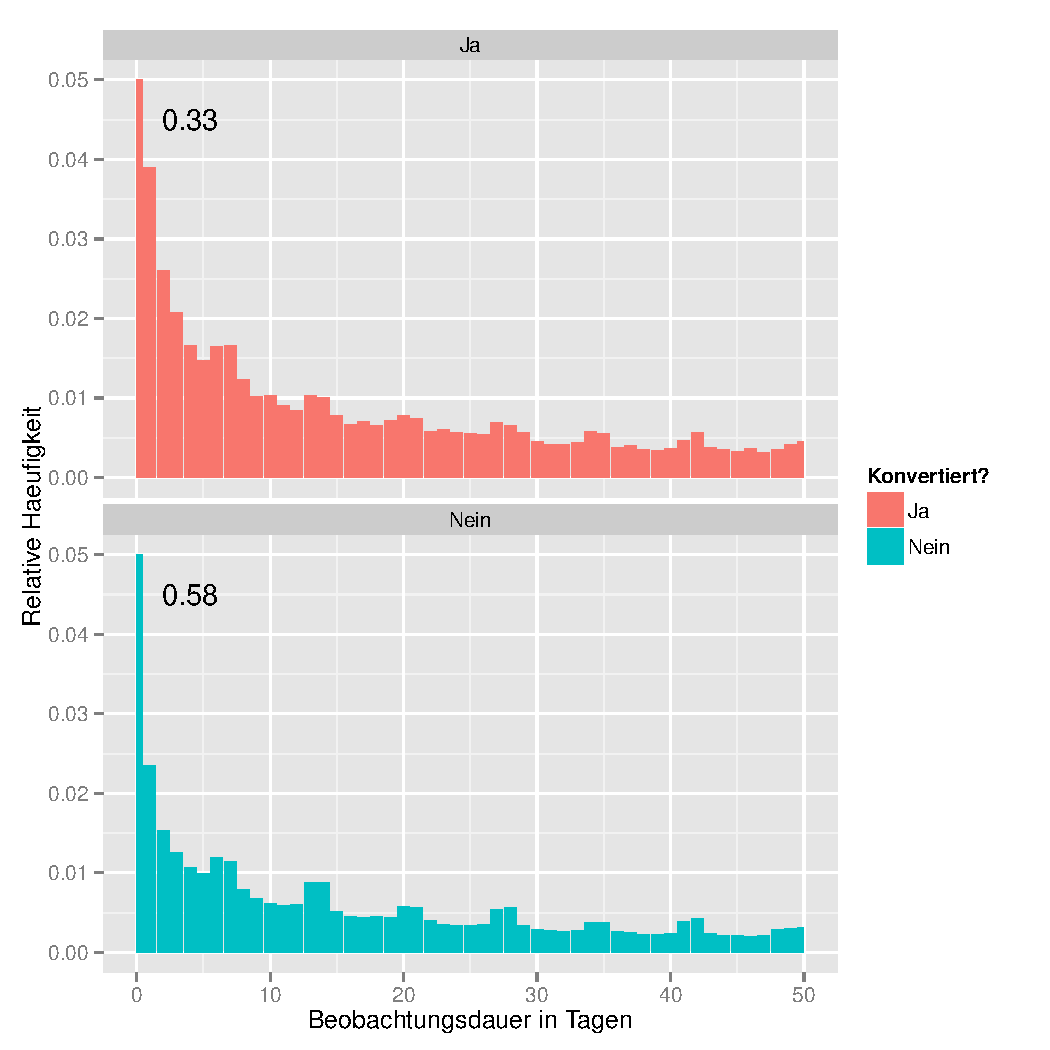
\includegraphics[scale=0.39]{timeSinceFirst_Last.pdf}
		\column{4cm}
			\begin{itemize}
				\item Verstrichene Zeit seit dem ersten Kontaktpunkt
				\item In der Abbildung wird nur der letzte Kontaktpunkt berücksichtigt
				\item Funnels mit Länge $1$ unberücksichtigt
				\item \textit{timeSinceLast}: Verstrichene Zeit seit dem vorherigen Kontaktpunkt
			\end{itemize}
	\end{columns}
\end{frame}

%\begin{frame}\frametitle{timeSinceLast}
	%\begin{columns}
		%\column{7cm}
			%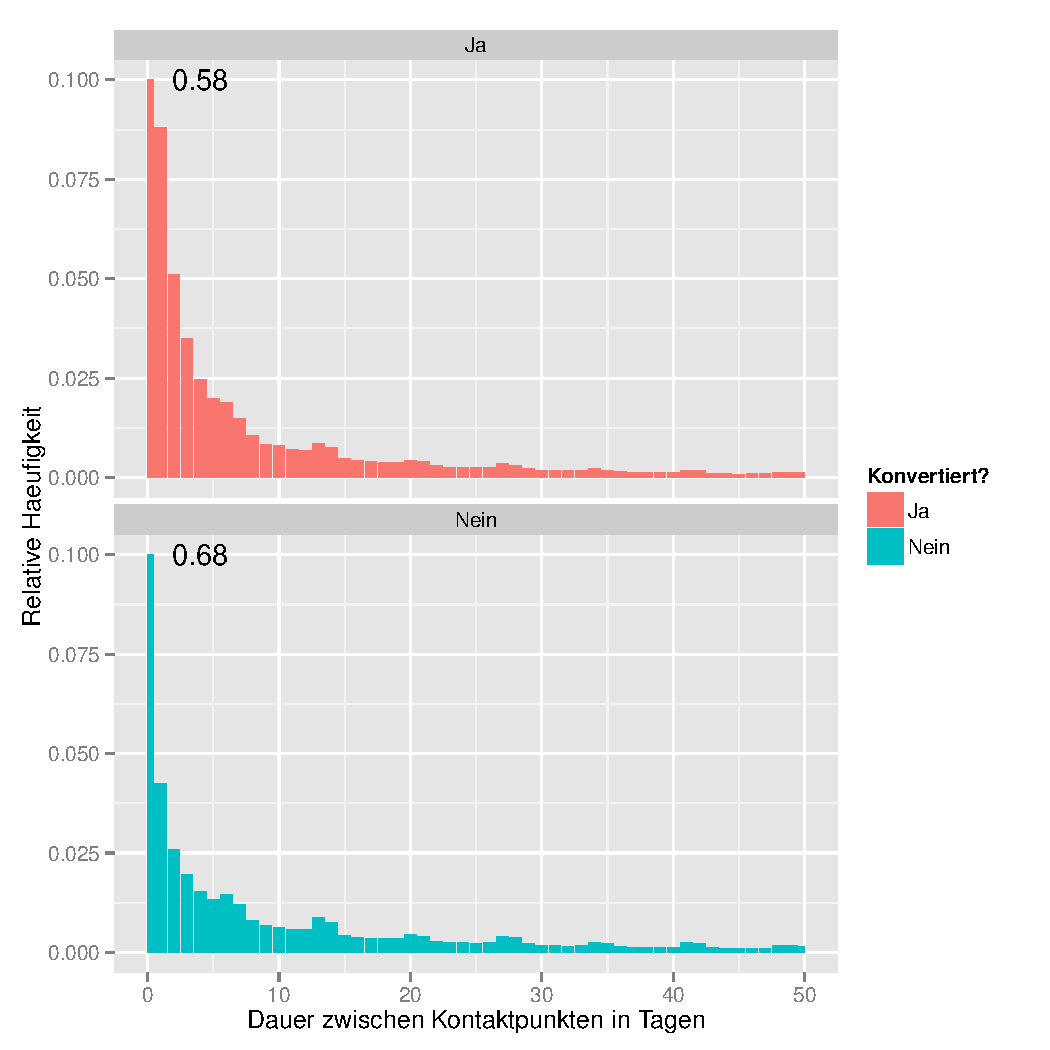
\includegraphics[scale=0.39]{timeSinceLast.pdf}
		%\column{4cm}
			%\begin{itemize}
				%\item 
			%\end{itemize}
	%\end{columns}
%\end{frame}

\begin{frame}\frametitle{freq}
	\begin{columns}
		\column{7cm}
			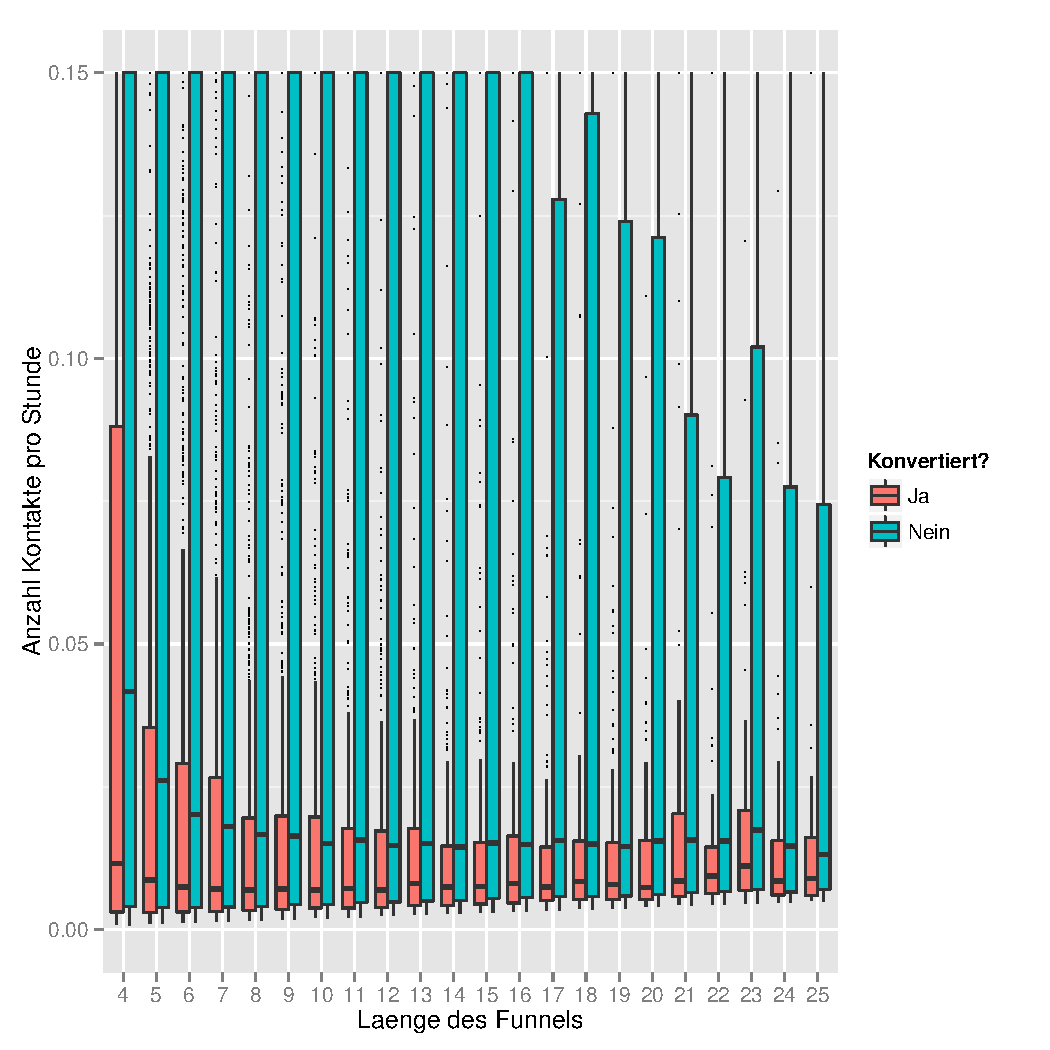
\includegraphics[scale=0.39]{freq.pdf}
		\column{4cm}
			\begin{itemize}
				\item \textit{funnelLength} dividiert durch Gesamt-Beobachtungsdauer in Stunden
				\item Frequenzen in nicht-konvertierten Funnels höher
			\end{itemize}
	\end{columns}
\end{frame}

\section{Methoden}

\begin{frame}\frametitle{Inhalt}
	\tableofcontents[currentsection,hideallsubsections]
\end{frame}

\subsection{Zeitdiskretes Survival-Modell}

\begin{frame}
	\begin{itemize}
		\item Zeit bis zu einem Ereignis $\Rightarrow$ Konvertierung oder Nicht-Konvertierung bzw. Rechtszensierung
		\item Positionen bilden Zeitachse des Modells $\Rightarrow$ Zeitdiskretes Modell
		%\item Stochastic Gradient Boosting mit Stümpfen als Basis-Lerner
		\item Zielvariable:	
			\begin{align*}
				y_{ip} =& \begin{cases} 1 & \text{Beobachtung } i \text{ konvertiert an Position } p\\
															 0 & \text{sonst} 
								 \end{cases}\\
								&p=1,...,25 \text{, } i=1,...,N_p 
			\end{align*}	
	\end{itemize}
\end{frame}

\begin{frame}
	\begin{itemize}
		%\item Zielvariable:	
			%\begin{align*}
				%y_{ip} =& \begin{cases} 1 & \text{Beobachtung } i \text{ konvertiert an Position } p\\
					%										 0 & \text{sonst} 
						%		 \end{cases}\\
							%	&p=1,...,25 \text{, } i=1,...,N_p 
			%\end{align*}	
		\item Hazardrate: 
			\begin{align*}
				\lambda_{ip} = P(y_{ip}=1|funnelLength_i \geq p, x_{ip})
			\end{align*}
		\item Logit-Modell: 
			\begin{align*}
				y_{ip}|x_{ip} &\stackrel{ind}{\sim} Bin(1, \lambda_{ip})  \\
				E(y_{ip}|x_{ip}) = P(y_{ip} = 1|x_{ip}) = \lambda_{ip} &= h(f_p(x_{ip})) = \frac{\exp(f_p(x_{ip}))}{1+\exp(f_p(x_{ip}))}
			\end{align*}
		\item Binomieller Verlust: 
			\begin{align*}
				L(y_{ip},f_p(x_{ip})) = -\sum_{i=1}^{N_p} (y_{ip} f_p(x_{ip}) + \ln(1+\exp(f_p(x_{ip}))))
			\end{align*}
	\end{itemize}
\end{frame}

%\begin{frame}
	%\begin{itemize}
		%\item Likelihood: 
			%\begin{align*}
				%L(\lambda_{ip}) &= \prod_{i=1}^{N_p} \lambda_{ip}^{y_{ip}} (1-\lambda_{ip})^{1-y_{ip}}
			%\end{align*}
		%\item Log-Likelihood: 
			%\begin{align*}
				%l(\lambda_{ip}) &= \ln(L(\lambda_{ip})) = \sum_{i=1}^{N_p} (y_{ip} \ln(\lambda_{ip}) + (1-y_{ip}) \ln(1-\lambda_{ip}))\\
				%&= \sum_{i=1}^{N_p} (y_{ip} f(x_{ip}) - \ln(1+\exp(f(x_{ip}))))
			%\end{align*}
		%\item Binomieller Verlust: 
			%\begin{align*}
				%L(y,f) = -yf + \ln(1+\exp(f))
			%\end{align*}
	%\end{itemize}
%\end{frame}

\begin{frame}
	\begin{itemize}
		\item Prädiktorfunktion:
			\begin{align*}
			f_p(x_{ip}) =&f_{weekday,p}(\text{weekday}_{ip}) +\\
								 &f_{hour,p}(\text{hour}_{ip}) +\\
								 &f_{campaign,p}(\text{campaign}_{ip}) +\\
								 &f_{campaignLast,p}(\text{campaign}_{i,p-1}) +\\
								 &f_{campaignLast2,p}(\text{campaign}_{i,p-2}) +\\
								 &f_{timeSinceLast,p}(\text{timeSinceLast}_{ip}) +\\
								 &f_{timeSinceFirst,p}(\text{timeSinceFirst}_{ip}) +\\
								 &\text{offset}(\hat{\lambda}_{i,p-1})
			\end{align*}
	\end{itemize}
\end{frame}

\begin{frame}\frametitle{Gradient Boosting - Pseudocode}
	\floatname{algorithm}{Algorithmus}
	%\begin{algorithm}
	%\caption{Gradient Boosting}\label{alg}
	%\label{gradboosting}
		\begin{algorithmic}
		\STATE Setze Startwert für $f_{0p}(x_{ip})$
		\FOR{$m=1:n.trees$}
			\STATE Setze $\lambda_{ip}(x_{ip}) = \frac{\exp(f_{m-1,p}(x_{ip}))}{1+\exp(f_{m-1,p}(x_{ip}))}$
			\FOR{$i=1:N_p$} 
				\STATE $r_{imp} = - \frac{\partial L(y_{ip},f_{m-1,p}(x_{ip}))}{\partial f_{m-1,p}(x_{ip})} = y_{ip} - \lambda_{ip}(x_{ip})$
			\ENDFOR
			%\STATE Fit a regression base learner to the pseudo-residuals $r_{im}$:
			\STATE $\theta_{mp} = \argmin_{\theta} \sum_{i=1}^{N_p} (r_{imp} - h(x_{ip}, \theta))^2$
			\STATE $\beta_{mp} = \argmin_{\beta} \sum_{i=1}^{N_p} L(y_{ip}, f_{m-1,p}(x_{ip}) + \beta h(x_{ip},\theta_{mp}))$
			\STATE $f_{mp}(x_{ip}) = f_{m-1,p}(x_{ip}) + \beta_{mp} h(x_{ip},\theta_{mp})$
		\ENDFOR
		\end{algorithmic}
	%\end{algorithm}
\end{frame}

\begin{frame}\frametitle{Parameter des Modells}
	\begin{itemize}
		\item Trainingsdaten machen Hälfte der gesamten Daten aus - stratifiziert bezüglich Transaction, Campaign, funnelLength
		\item $n.trees=3000$
		\item $cv.folds=5$
		\item Shrinkage-Parameter: $\mu = 0.01 \Rightarrow f_{mp}(x_{ip}) = f_{m-1,p}(x_{ip}) + \mu \beta_{mp} h(x_{ip},\theta_{mp})$
		\item $interaction.depth=1$
		\item $bag.fraction=0.5 \Rightarrow$ \textbf{Stochastic} Gradient Boosting
	\end{itemize}
\end{frame}

\begin{frame}\frametitle{Output des Modells}
	\begin{itemize}
		\item $\hat{f}_p(x_{ip})$ für jede Beobachtung $i$ und jede Position $p$
			\begin{align*}
				\hat{\lambda}_{ip} = \frac{\exp(\hat{f}(x_{ip}))}{1+\exp(\hat{f}(x_{ip}))}
			\end{align*}
		\item Relative Wichtigkeit der Features:
			\begin{align*}
				\hat{I}_{jp} &= \sqrt{\frac{1}{M} \sum_{m=1}^{n.trees} \hat{i}_{mp} 1_{jmp}}
			\end{align*}
		\item Marginale Effekte der Features:
			\begin{align*}
				\bar{f}_{jp}(x_{jp}) = \frac{1}{N} \sum_{i=1}^{N_p} \hat{f}(x_{jp},x_{i,\backslash j,p})
			\end{align*}
		\item ROC-Kurve und AUC
	\end{itemize}
\end{frame}

\subsection{Sequential Pattern Mining}

\begin{frame}
	\begin{itemize}
		\item Menge von Items $I = \{a, b, c, d, e\}$ $\Rightarrow$ Kampagnen
		\item Datenbank: $[ID 1, <abcdbaae>]$; $[ID 2, <edcaa>]$
		\item 4-Sequenz $s = b\rightarrow b\rightarrow a\rightarrow e$
		\item Support einer Sequenz: Anteil der IDs, die $s$ unterstützen
		\item SPADE-Algorithmus findet häufige Sequenzen, deren Support größer als ein festgelegter minimaler Support ist
		\item Seperate Anwendung auf konvertierte und nicht-konvertierte Funnels
	\end{itemize}
\end{frame}

\subsection{Visualisierung anhand eines Netzwerkes}

\begin{frame}
	\begin{itemize}
		\item Geordneter Graph $G=(V,E)$ besteht aus Menge $V$ von Knoten und Menge $E$ von Kanten
		\item Kante $e_i \in E$ besteht aus geordneten Paar von zwei Knoten $(v_j,v_k)$, wobei $v_j,v_k \in V$
		\item Startpunkt $\rightarrow$ $17$ Kampagnen der ersten Position $\rightarrow$ $Succ\_1$, $Fail\_1$ und $17$ Kampagnen der zweiten Position $\rightarrow$ $Succ\_2$, $Fail\_2$ und $17$ Kampagnen der dritten Position $\rightarrow$ ...
		\item Kanten sind bezüglich der Anzahl der Nutzer gewichtet
		\item Relative Ausgänge: relative Häufigkeiten der Kanten, wobei die zugrundeliegende Menge die Summe aller Nutzer ist, die einen Knoten verlassen
		\item Relative Eingänge: relative Häufigkeiten der Kanten, wobei die zugrundeliegende Menge die Summe aller Nutzer ist, die in einen Knoten gehen
	\end{itemize}
\end{frame}

\begin{frame}
	\begin{itemize}
		\item \textit{R}-Paket \textit{rgexf} $\rightarrow$ \textit{gexf}-Datei $\rightarrow$ \textit{Gephi}
		\item Berechnung der räumlichen Anordnung der Knoten und Kanten anhand von Algorithmen (z.B. \textit{Force Atlas 2})
		\item Manuelle Bearbeitung für die Präsentation von Ergebnissen
		\item Interaktives Arbeiten mit dem Netzwerk in \textit{Gephi} möglich $\rightarrow$ Tutorial dazu im Bericht
	\end{itemize}
	\centering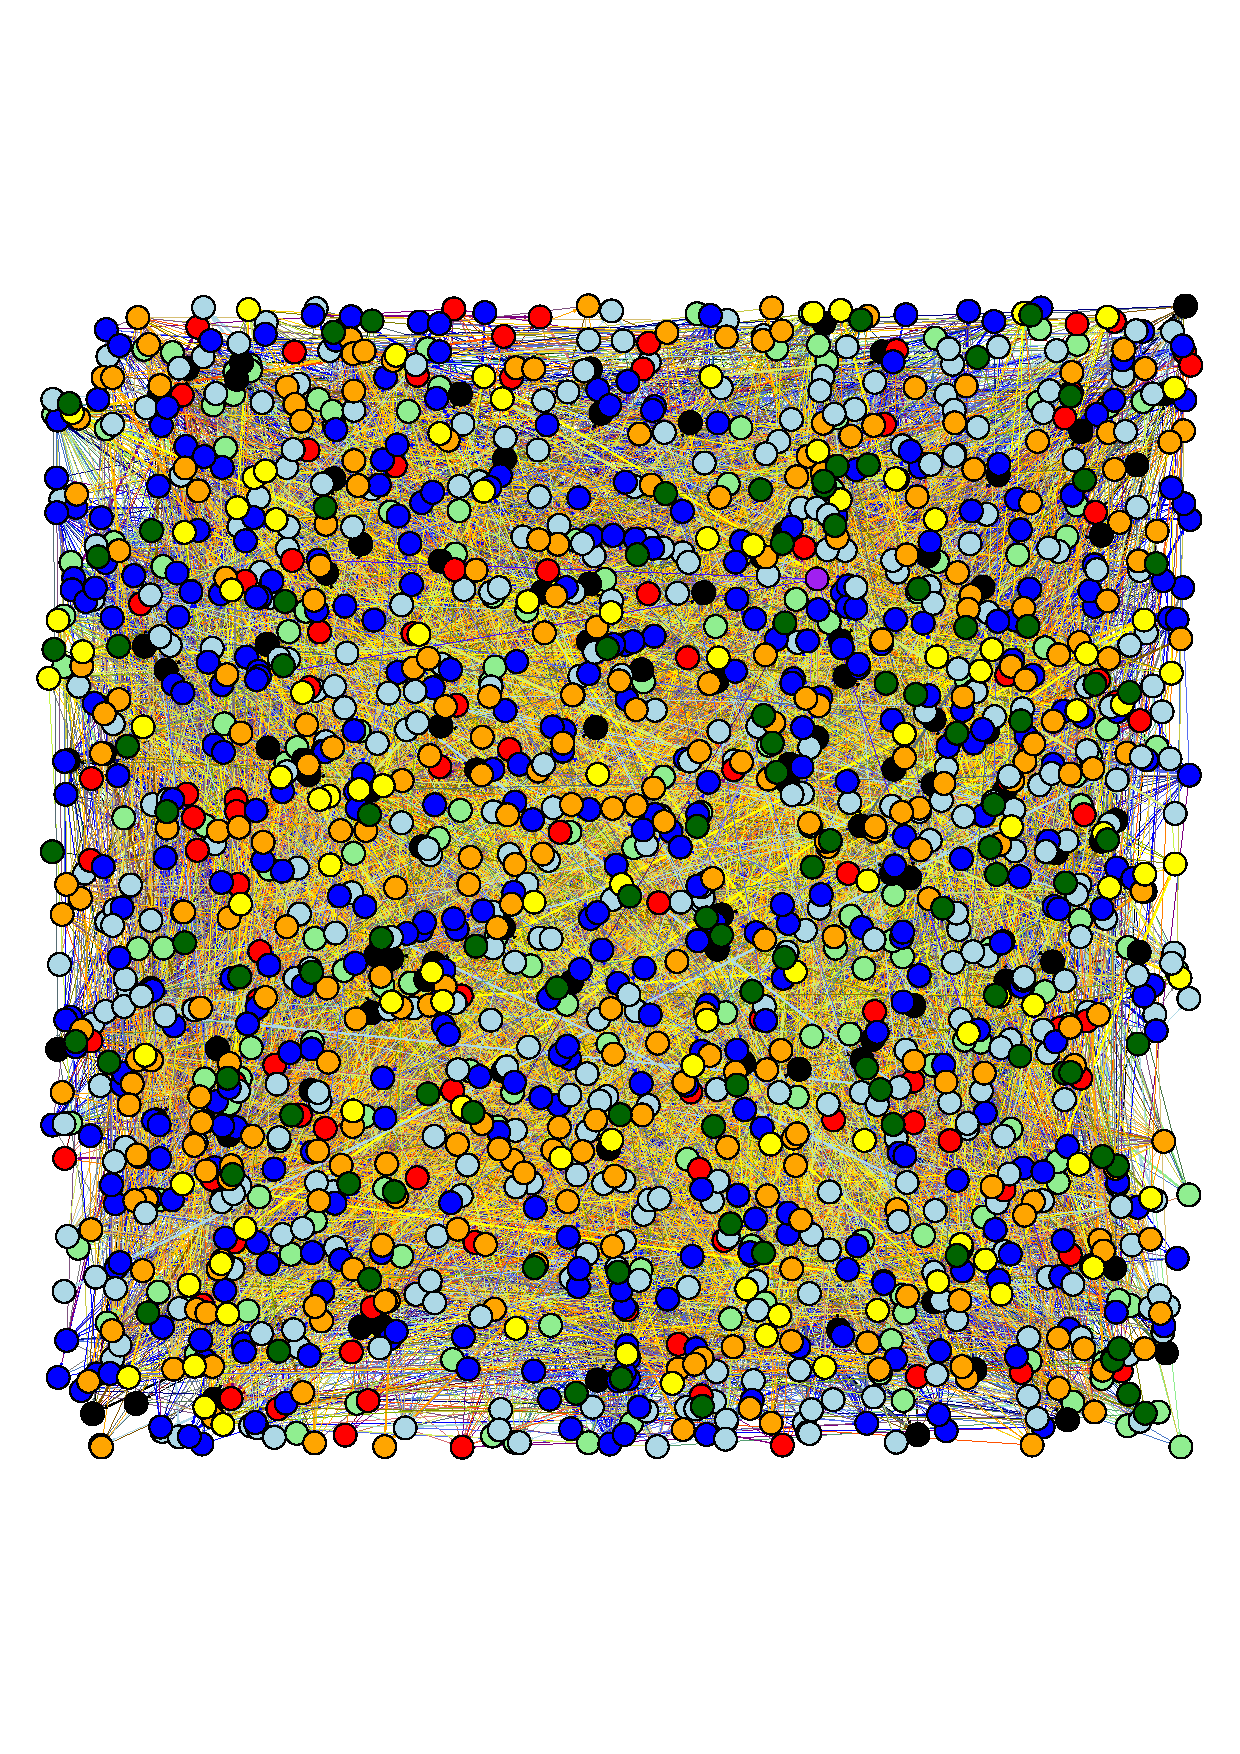
\includegraphics[scale=0.2]{graphbegin.pdf}
\end{frame}

\section{Ergebnisse}\label{ergebnisse}

\subsection{Zeitdiskretes Survival-Modell}

Die in diesem Kapitel präsentierten Ergebnisse basieren jeweils auf der bestmöglichen Anzahl an Iterationen. Diese wurden mittels $5$-facher Kreuzvalidierung ermittelt und sind in Abbildung \ref{best_iter} dargestellt. Auf der $x$-Achse ist die Position von $1$ bis $25$ aufgetragen und auf der $y$-Achse die Optimale Iterationsanzahl, die durch $n.trees = 3000$ nach oben begrenzt ist. Es ist zu erkennen, dass für die Positionen $1$ bis $4$ über $2500$ Stümpfe für die Ergebnisse verwendet werden. Dann fällt die Kurve sehr schnell ab bis sie sich bei ungefähr $500$ Iterationen einpendelt. Dieser Abfall ist dadurch zu erklären, dass mit steigender Position die Datenmenge sinkt.
\begin{figure}[H]
	\centering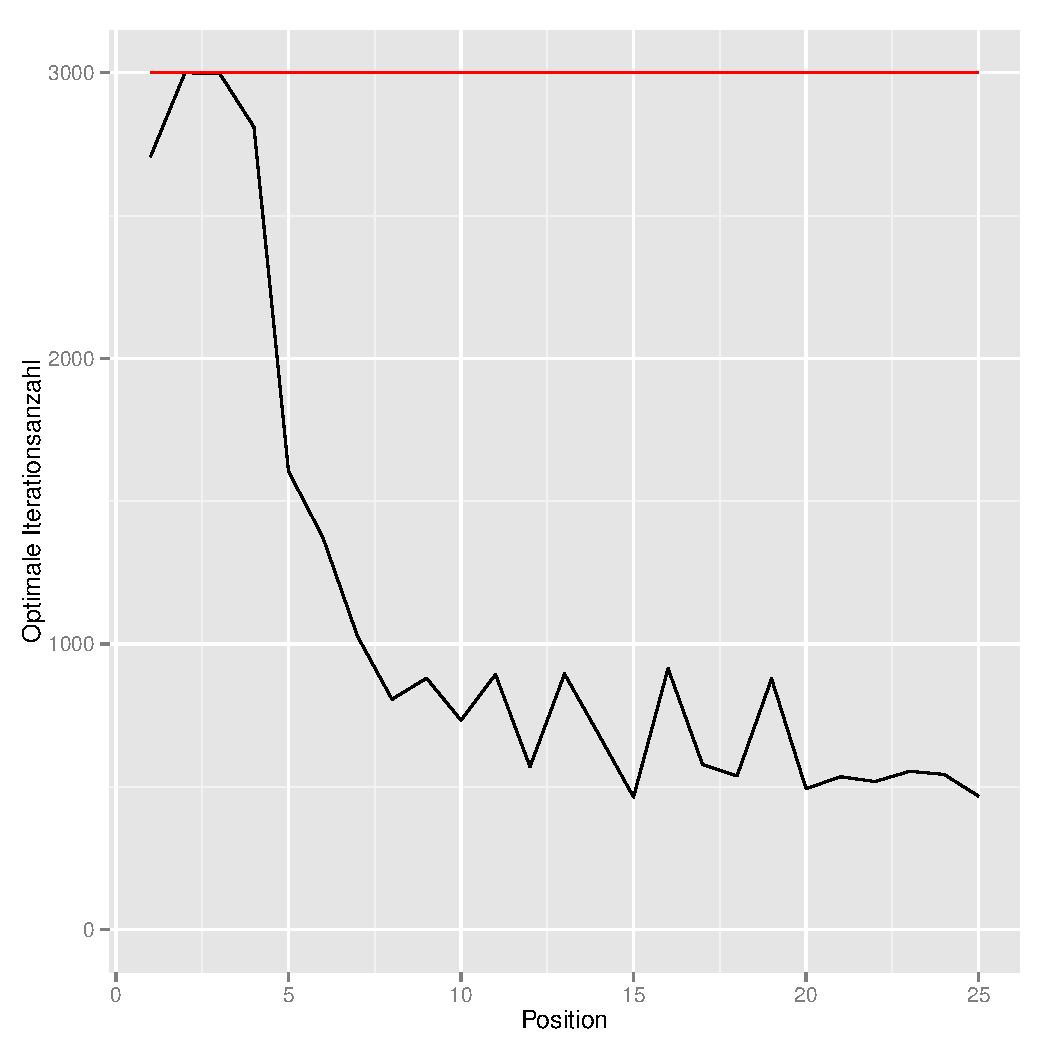
\includegraphics[scale=0.5]{bestIter.pdf}\caption[Optimale Iterationsanzahl]{Optimale Iterationsanzahl des Stochastic Gradient Boosting}\label{best_iter}
\end{figure}
Der relative Einfluss der Features gibt dessen Wichtigkeit bei der Erstellung der Prädiktorfunktion an und ist in Abbildung \ref{variable_importance} dargestellt. Auf der $x$-Achse ist erneut die Position aufgetragen und auf der $y$-Achse der relative Einfluss. Der relative Einfluss aller Features an einer Position ergibt summiert jeweils $100$ und die Balken sind der Größe nach geordnet, das heißt die wichtigsten Variablen sind unten abgebildet. Die Farben der Balken werden in der Legende rechts neben der Abbildung erläutert.\\
An Position $1$ sind nur drei Features vorhanden, wobei $Campaign$, das heißt die Art des Kontaktpunktes, für circa $90 \%$ der Minimierung der Verlustfunktion verantwortlich ist. Die Variablen $Hour$ und $Weekday$ haben kaum Einfluss. An Position $2$ ist die Kampagne immer noch das stärkste Feature, wobei hier auch die Kampagne des ersten Kontaktpunktes und die Zeit, die seit dem ersten Kontaktpunkt vergangen ist, Einfluss haben.\\
\begin{figure}[H]
	\centering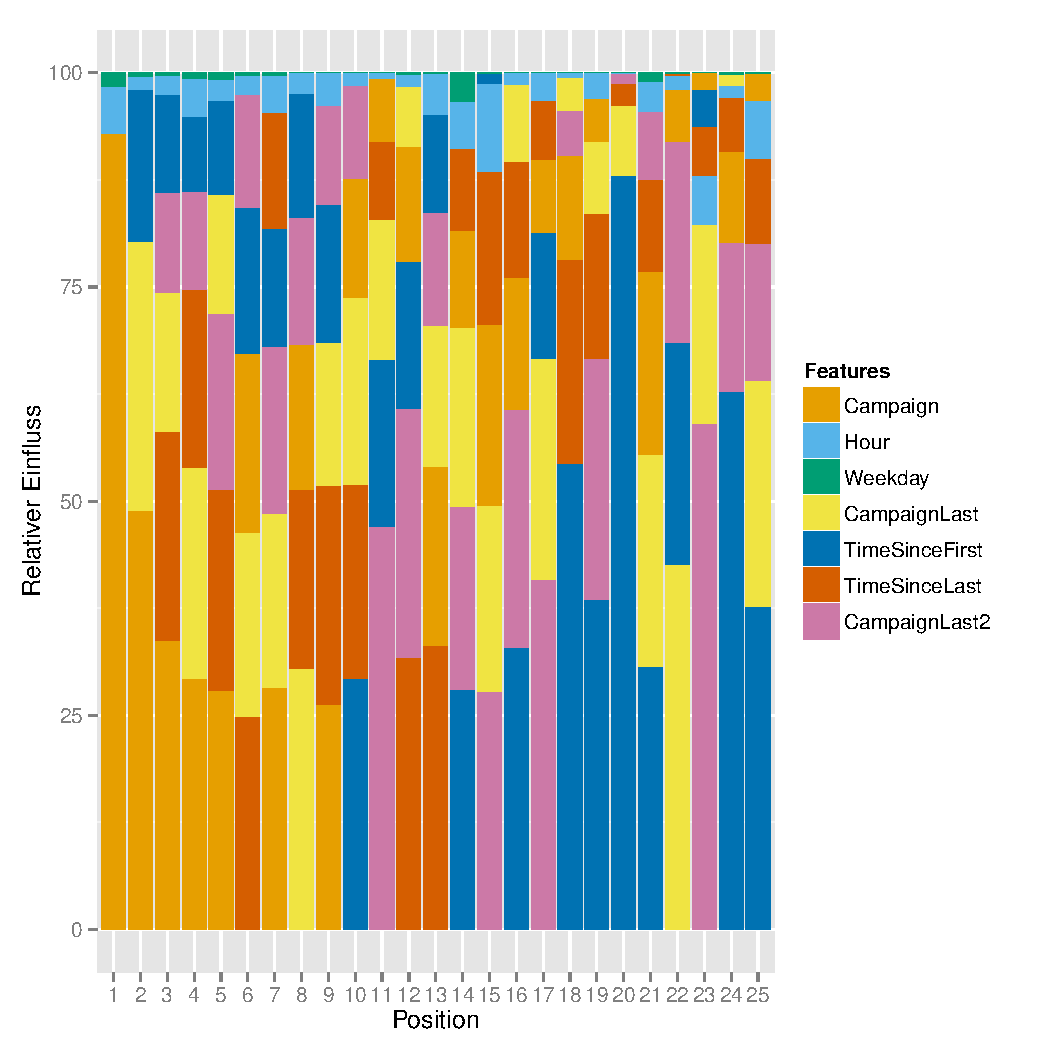
\includegraphics[scale=0.9]{variableImportance.pdf}\caption{Wichtigkeit der Variablen}\label{variable_importance}
\end{figure}
An den Positionen $8$ und $22$ hat die Kampagne des letzten Kontaktpunktes den stärksten Einfluss und damit selbstverständlich auch einen höheren Einfluss als die Kampagne des aktuellen Kontaktpunktes, die insbesondere an den höheren Positionen oft nur noch einen geringen Einfluss hat. Mit steigender Position wird auch die Kampagne des vorletzten Kontaktes wichtiger und ist manchmal das wichtigste Feature. Die Zeit, die seit dem vorherigen Kontaktpunkt vergangen ist, ist bereits an Position $3$ zweitwichtigstes Feature und spielt auch für die folgenden Positionen eine Rolle. Später nimmt die Wichtigkeit dieses Features allerdings ab und die Zeit, die seit dem ersten Kontaktpunkt vergangen ist, wird bedeutend wichtiger. Die Features $Hour$ und $Weekday$ spielen positionsübergreifend kaum eine Rolle.\\
Nachdem die Wichtigkeit der Variablen für die Klassifizierung in konvertierte und nicht-konvertierte Funnel präsentiert wurde, ist nun die Art dieses Einflusses interessant. Dieser wird im folgenden für einige Positionen dargestellt, wobei die Variablen dafür nach positionsspezifischer Wichtigkeit ausgesucht werden und das Augenmerk vor allem auf die niedrigeren Positionen fällt, da dort mehr Daten vorhanden sind. Folglich werden die Features $Hour$ und $Weekday$ garnicht präsentiert, das sie kaum einen Einfluss haben. Die Kampagne des vorletzten Kontaktpunktes $CampaignLast2$ wird an dieser Stelle ebenfalls nicht berücksichtigt, da die Ergebnisse für $Campaign$ beziehungsweise $CampaignLast$ oft sehr ähnlich sind. Im elektronischen Anhang sind die marginalen Effekte aller Features für jeweils jede Position zu finden.\\
In Abbildung \ref{marg_eff_campaign} sind die marginalen Effekte der Variable \textit{Campaign} für die Positionen eins bis vier, von links oben nach rechts unten, aufgetragen. \textit{Campaign} ist an den ersten vier Positionen das wichtigste Feature. Mit steigender Position verliert die Variable deutlich an Einfluss. Auf der $x$-Achse ist die Art des aktuellen Kontaktpunnktes aufgetragen und auf der $y$-Achse der Marginale Effekt.\\
An Position eins haben die Kampagnen \textit{Affiliate - Rest}, \textit{E-Mailing} und \textit{SEM - Brand} im Vergleich zu den restlichen Kampagnen einen starken, positiven Einfluss auf die Konvertierungswahrscheinlichkeit.\\
Das heißt das Bereitstellen von Zinsvergleichen, welche das Zinsangebot der Interhyp AG mit deren Wettbewerbern im Vergleich darstellt, durch die Partner unter \textit{Affiliate - Rest} scheint oft an Position $1$ bereits zur Konvertierung zu führen. Die Partner unter \textit{Affiliate - Partnerprogramm}, die hauptsächlich Rechner der Interhyp AG auf ihren Seiten einbinden, teilweise aber auch Banner schalten oder Verlinkungen in Texten unterbringen, haben an Position $1$ einen deutlich geringeren Effekt. \textit{E-Mailing} sind Mails, die an Interessenten, die schon einen Antrag gestellt haben oder ein Infopaket angefordert hatten, versendet werden. Da dieses Klientel sich offentsichtlich bereits intensiv mit einer Baufinanzierung beschäftigt hat, macht es Sinn, dass diese Mails schon nach wenigen Kontakten häufig zu einer Konvertierung führen und dieser Effekt für spätere Positionen schwächer ist. SEM sind bezahlte Suchergebnisse, hauptsächlich auf Google. \textit{SEM - Brand} bedeutet, dass der Suchbegriff das Wort \textit{Interhyp} enthielt. Dieser Effekt ist deutlich größer als für \textit{SEM - Generisch} beziehungsweise \textit{SEM - Remarketing}, wobei ersteres bedeutet, dass etwas wie \textit{Baufinanzierung} gesucht wurde und zweiteres, dass der potentielle Kunde bereits zuvor auf der Seite von Interhyp war und deshalb nochmal eine Einblendung mit Werbung der Interhyp AG bekommen hat.\\
An Position $2$ stechen neben \textit{Affiliate - Rest}, \textit{SEM - Brand} und \textit{E-Mailing} auch \textit{Direct} und \textit{Generic} durch ihre Marginalen Effekte leicht hervor. \textit{Direct} bedeutet, dass jemand im Browser direkt \textit{www.interhyp.de} eingegeben hat und \textit{Generic}, dass jemand über einen unbezahlten Link zur Interhyp kam.
Für die Positionen $3$ und $4$ ist vor allem \textit{Generic} wichtig. \textit{Display}, \textit{Social Media}, \textit{SEO} sowie die Kooperationen spielen, neben den bereits erwähnten, keine große Rolle für die ersten vier Positionen.
\begin{figure}[H]
	\centering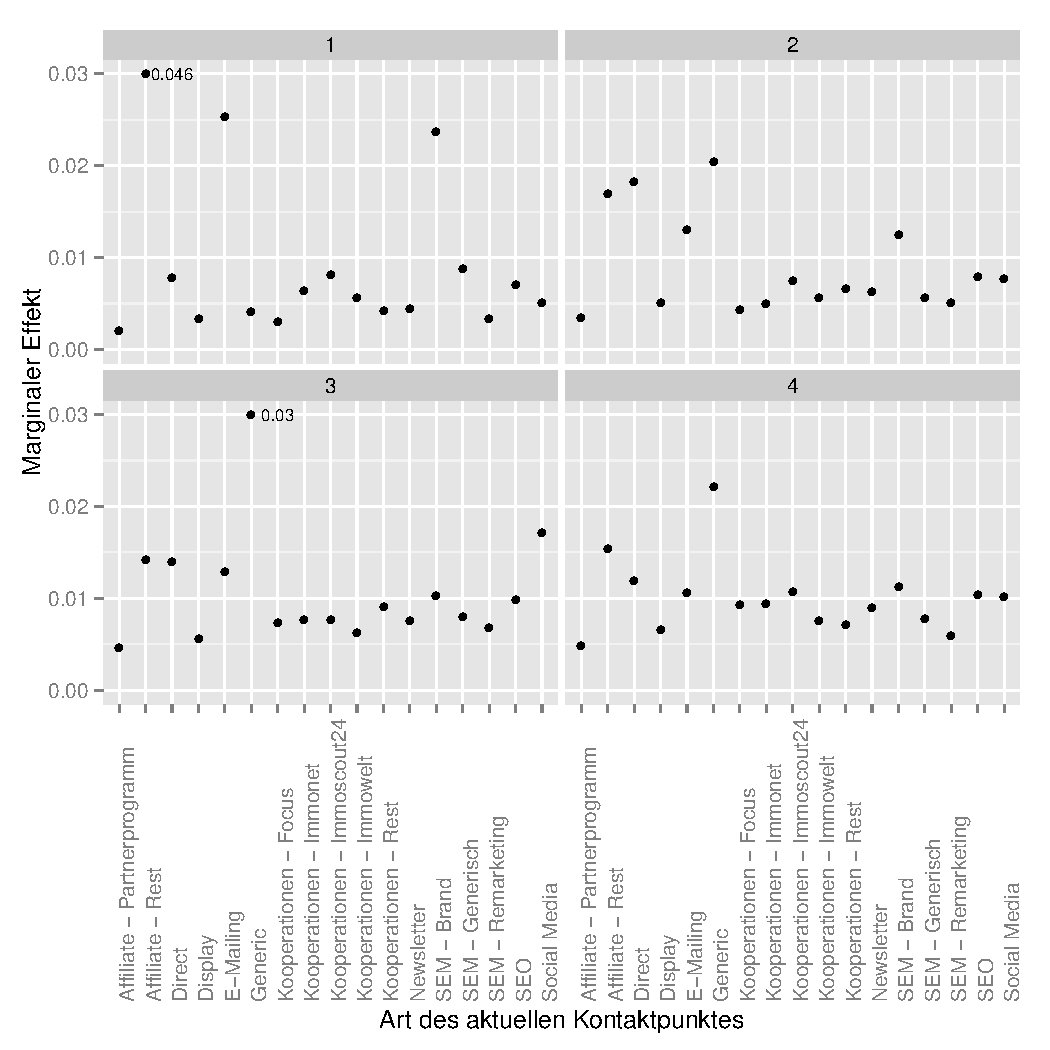
\includegraphics[scale=0.75]{marg_eff_campaign.pdf}\caption[Marginaler Effekt von \textit{Campaign}]{Marginaler Effekt des Features \textit{Campaign} an den Positionen $1$, $2$, $3$ und $4$}\label{marg_eff_campaign}
\end{figure}
An den Positionen $4$, $6$ und $7$ ist \textit{CampaignLast} das zweitwichtigste Feature sowie an Position $8$ das wichtigste. Dessen marginalen Effekte sind in Abbildung \ref{marg_eff_campaignLast} dargestellt. Hier heben sich teilweise die selben Kategorien hervor, wobei die Unterschiede zwischen den Kampagnen kleiner sind. Überraschend ist, dass hier auch \textit{Social Media} einen starken Effekt hat. Allerdings liegen hierfür kaum Daten vor, wie in Abbildung \ref{campaign} zu erkennen ist.\\
\begin{figure}[H]
	\centering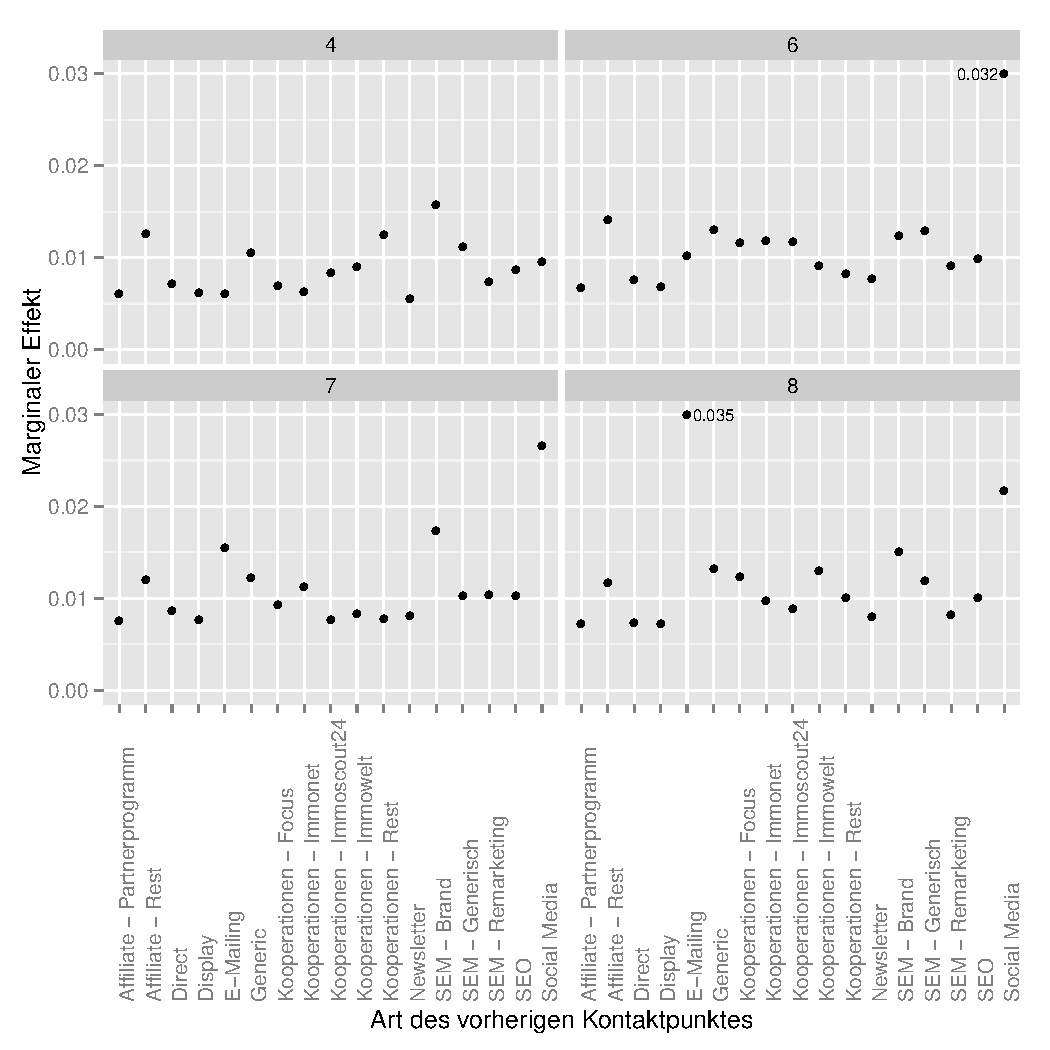
\includegraphics[scale=0.75]{marg_eff_campaignLast.pdf}\caption[Marginaler Effekt von \textit{CampaignLast}]{Marginaler Effekt des Features \textit{CampaignLast} an den Positionen $4$, $6$, $7$ und $8$}\label{marg_eff_campaignLast}
\end{figure}
Das Feature \textit{TimeSinceFirst} ist an den Positionen $10$ und $14$ das wichtigste sowie an Position $11$ und $12$ das zweit- beziehungsweise drittwichtigste. \textit{TimeSinceLast} ist an den Positionen $6$, $12$ und $13$ das wichtigste Feature und an Position $8$ das zweitwichtigste Feature. Die marginalen Effekte für diese Positionen sind in Abbilung \ref{marg_eff_time} dargestellt, wobei diese an anderen Positionen ähnlich aussehen. Auf der $x$-Achse ist die Zeit in Tagen aufgetragen und auf der $y$-Achse die Marginalen Effekte. Für beide Features und alle Positionen steigen die marginalen Effekte mit der Zeit, wobei der Effekt bei \textit{TimeSinceLast} etwas größer ist.\\
Dass die Konvertierungswahrscheinlichkeit bei zeitlich längeren Funnels höher ist, könnte man dadurch erklären, dass die Entscheidung für den Bau eines Hauses oder ähnlichem und das damit verbundene Ausfüllen eines Online-Antrages viel Zeit in Anspruch nimmt. Dass für die Zeit seit des vorherigen Kontaktes der selbe Effekt auftritt, könnte man ähnlich erklären. Bei der Entscheidung für eine Baufinanzierung sind viele Dinge zu beachten. So erscheint es plausibel, dass sich interessierte Kunden eine längere Zeit auch offline mit dem Thema beschäftigen und später wieder online den Kontakt zur Interhyp AG suchen.
\begin{figure}[H]
	\centering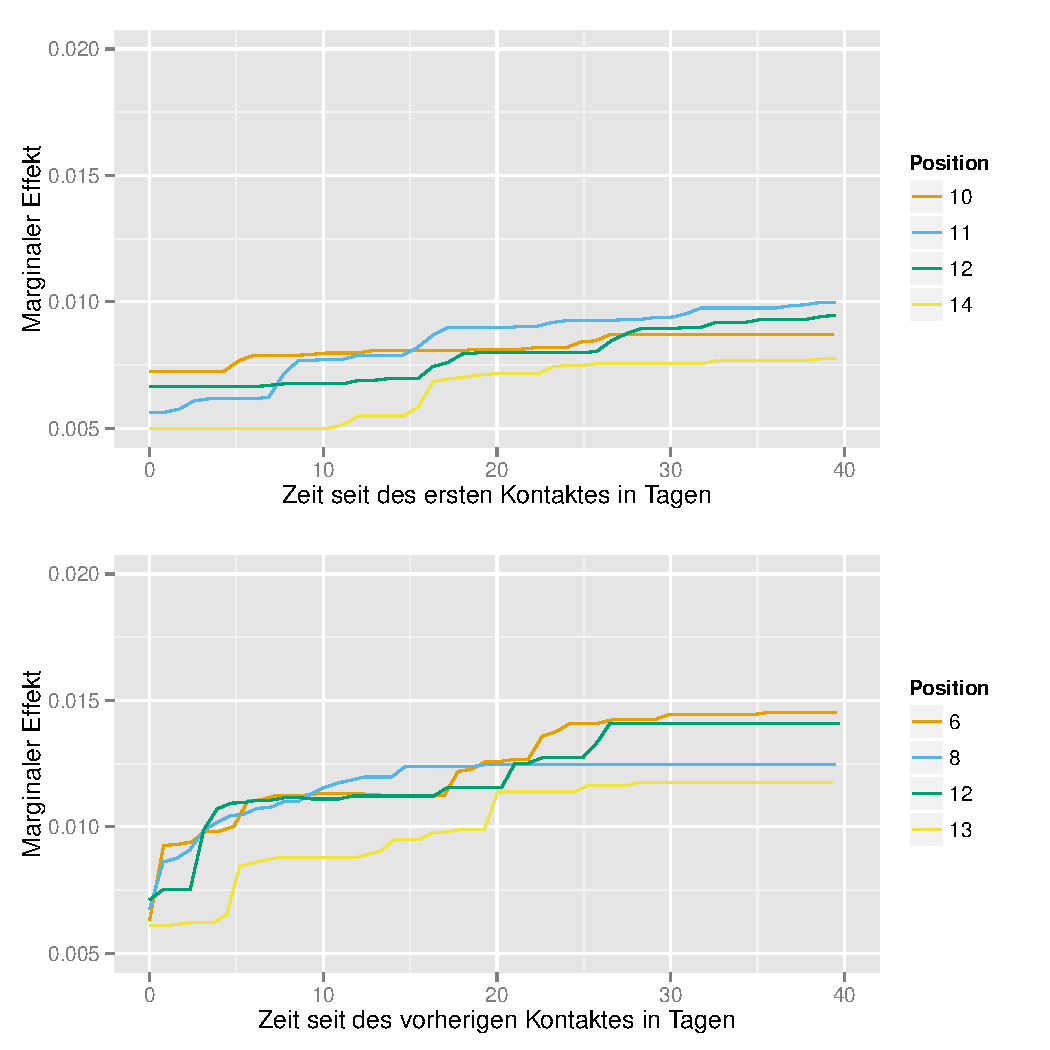
\includegraphics[scale=0.75]{marg_eff_time.pdf}\caption[Marginaler Effekt von \textit{TimeSinceFirst} und \textit{TimeSinceLast}]{Marginaler Effekt des Features \textit{TimeSinceFirst} an den Positionen $10$, $11$, $12$ und $14$ (oben) und des Features \textit{TimeSinceLast} an den Positionen $6$, $8$, $12$ und $13$ (unten)}\label{marg_eff_time}
\end{figure}
Bis hierhin wurden die Ergebnisse des, auf den Trainingsdaten geschätzten, Modells vorgestellt. Nun soll das Modell auf die Testdaten angewendet werden, um die Prognosegüte zu beurteilen.\\
Wenn man die geschätzte Prognosefunktion auf die Testdaten anwendet, bekommt man für jede Position und jede ID aus den Testdaten die Hazardrate, das heißt die Wahrscheinlichkeit an einer bestimmten Position zu konvertieren. Diese sind sowohl für konvertierte als auch nicht-konvertierte Funnels sehr niedrig, da die absolute Anzahl an nicht-konvertierten Funnels deutlich überwiegt. Um die Prognosegüte des Modells näher zu betrachten wurde deshalb für jede Position eine ROC-Kurve berechnet. Diese sind in Abbildung \ref{roc} für vier Positionen beispielhaft dargestellt.\\
%An Position $1$ ist dieser Unterschied noch nicht sehr deutlich. Dies kann daran liegen, dass hier nur die Features \textit{Campaign}, \textit{Hour} und \textit{Weekday} einfließen und noch keine Informationen über vorherige Positionen vorliegen. Von dort steigen die Hazardraten an, wobei dieser Anstieg in den konvertierten Funnels deutlich stärker ist als in den nicht-konvertierten. Ab Position $6$ werden die Konvertierungswahrscheinlichkeiten wieder geringer, wobei immer noch ein deutlicher Unterschied zwischen konvertiert und nicht-konvertiert zu erkennen ist.\\
Auf der $x$-Achse ist der Anteil der nicht-konvertierten Funnels, die als konvertiert vorhergesagt wurden aufgetragen und auf der $y$-Achse der Anteil der konvertierten Funnels, die auch als konvertiert vorhergesagt wurden. Je weiter die ROC-Kurve also oberhalb der roten Diagonalen liegt, desto besser kann das Modell zwischen konvertierten und nicht-konvertierten Funnels trennen. Für Position $3$ liegt die Kurve für alle Punkte überhalb der Kurve von Position $1$. Dies ist dadurch zu erklären, dass an Position $3$ mehr Informationen zur Erstellung des Modells verwendet werden als an Position $1$. Für Position $15$ und $22$ ist das Modell schlechter als an Position $3$. Die Kurven für die späteren Positionen sind deutlich rauher. Dies ist darauf zurück zu führen, dass dort weniger Datenpunkte vorhanden sind. Durch das Einbringen des Offsets kann die Prognoseleistung des Modells allerdings halbwegs konstant gehalten werden.\\
\begin{figure}[H]
	\centering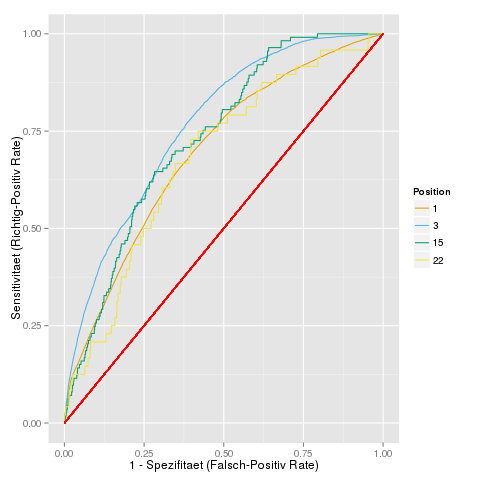
\includegraphics[scale=0.5]{roc.png}\caption[ROC-Kurve]{ROC-Kurve für die Positionen $1$, $3$, $15$ und $22$}\label{roc}
\end{figure}
Dies ist in Abbildung \ref{auc} noch deutlicher zu erkennen. Hier ist die Fläche unterhalb der ROC-Kurve (AUC) für jede Position abgebildet. Dieser Wert fällt zwischen Position $15$ und $22$ unter $0.75$ ab, hält sich ansonsten aber relativ konstant auf $0.75$. Das heißt die Wahrscheinlichkeit, dass bei einer konvertierten Beobachtung die Hazardrate größer ist als bei einer nicht-konvertierten Beobachtung ist positionsübergreifend circa $0.75$.
\begin{figure}[H]
	\centering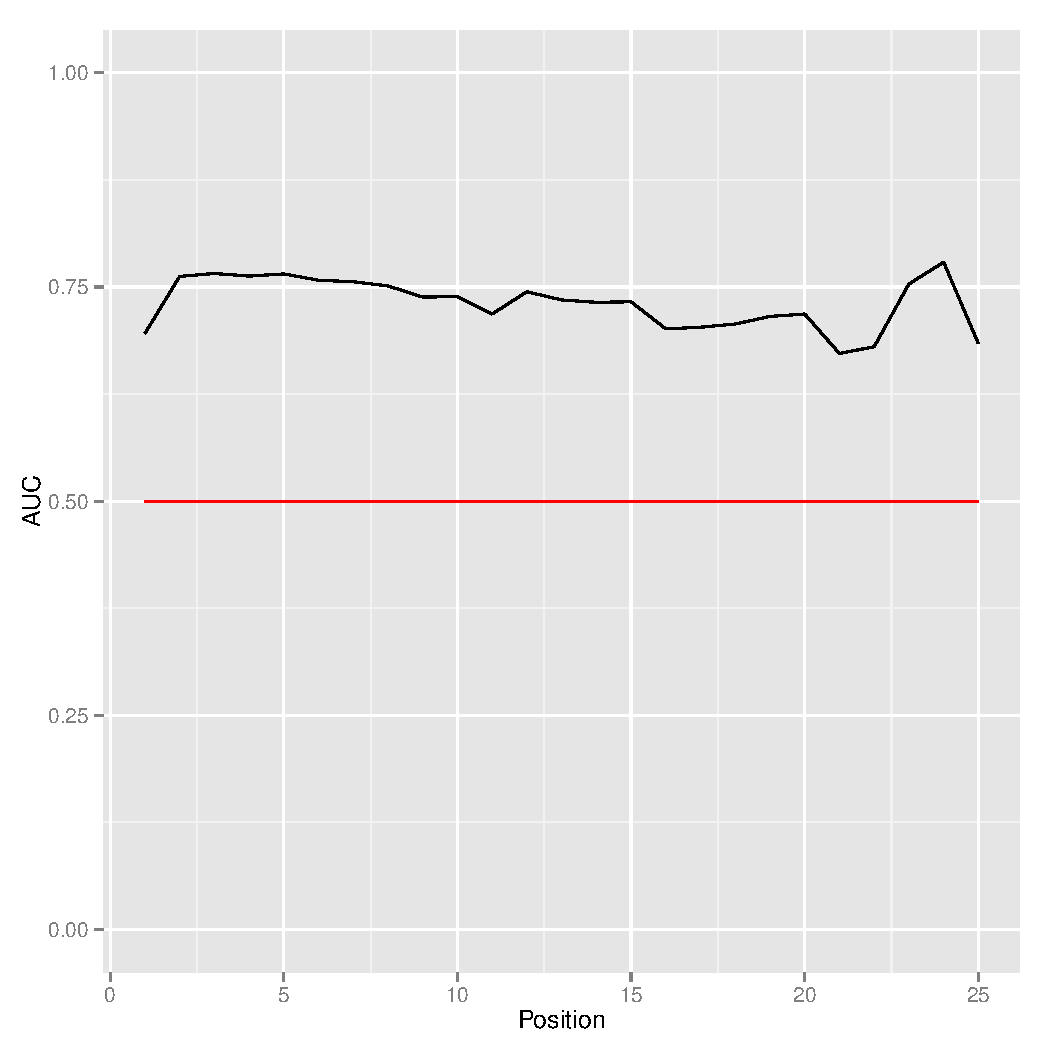
\includegraphics[scale=0.75]{auc.pdf}\caption[AUC-Wert]{AUC für alle Positionen}\label{auc}
\end{figure}

\subsection{Sequential Pattern Mining}\label{ergspm}

Der in Kapitel \ref{spm} beschriebene Algorithmus wurde zunächst seperat auf alle konvertierten sowie nicht-konvertierten Funnels angewendet. Dabei wurden Funnels mit der Länge eins ausgeschlossen, da in diesen offentsichtlich keine interessanten Sequenzen enthalten sein können. Der minimale Support wurde auf $0.05$ gesetzt, so dass nur Sequenzen, die in mindestens $5 \%$ aller Funnels vorkommen, als Ergebnis ausgegeben werden. In Abbildung \ref{spm_all} sind diese Sequenzen geplottet, wobei auf der $x$-Achse der Suppport aufgetragen ist und die Sequenzen anhand des Supports der Sequenzen in den konvertierten Funnels absteigend geordnet sind. An den Stellen, wo keine Balken geplottet sind, war der Support kleiner als $0.05$. Die Namen der Kampagnen sind teilweise abgekürzt, um die Darstellung zu verbessern. \textit{AffPar} steht für \textit{Affiliate - Partnerprogramm}, \textit{Dir} für \textit{Direct} und \textit{Dis} für \textit{Display}. Außerdem ist zu beachten, dass die Sequenzen nicht exakt in der dargestellten Weise in den Funnels vorkommen müssen, sondern auch Abstände zwischen den aufeinanderfolgenden Kampagnen erlaubt sind.\\
Der Support von Sequenzen der Länge eins, wie \textit{<\{Dir\}>} oder \textit{<\{SEO\}>}, geben lediglich an, wie groß der Anteil der Funnels ist, die diese Kampagne mindestens einmal enthalten. Interessanter sind Sequenzen, die mindestens zwei Kampagnen enthalten. Hier fällt auf, dass Sequenzen mit wiederholtem \textit{Direct}-Kontakt in den konvertierten Funnels stärker sind. Umgekehrt sind  Sequenzen mit wiederholtem \textit{Affiliate - Partnerprogramm}-Kontakt in den nicht-konvertierten Funnels stärker. Allerdings haben die Sequenzen insgesamt einen sehr geringen Support. Das liegt vor allem daran, dass die Daten zu großem Teil aus sehr kurzen Funnels bestehen (siehe Abbildung \ref{funnelLength}).\\
\begin{figure}[H]
	\centering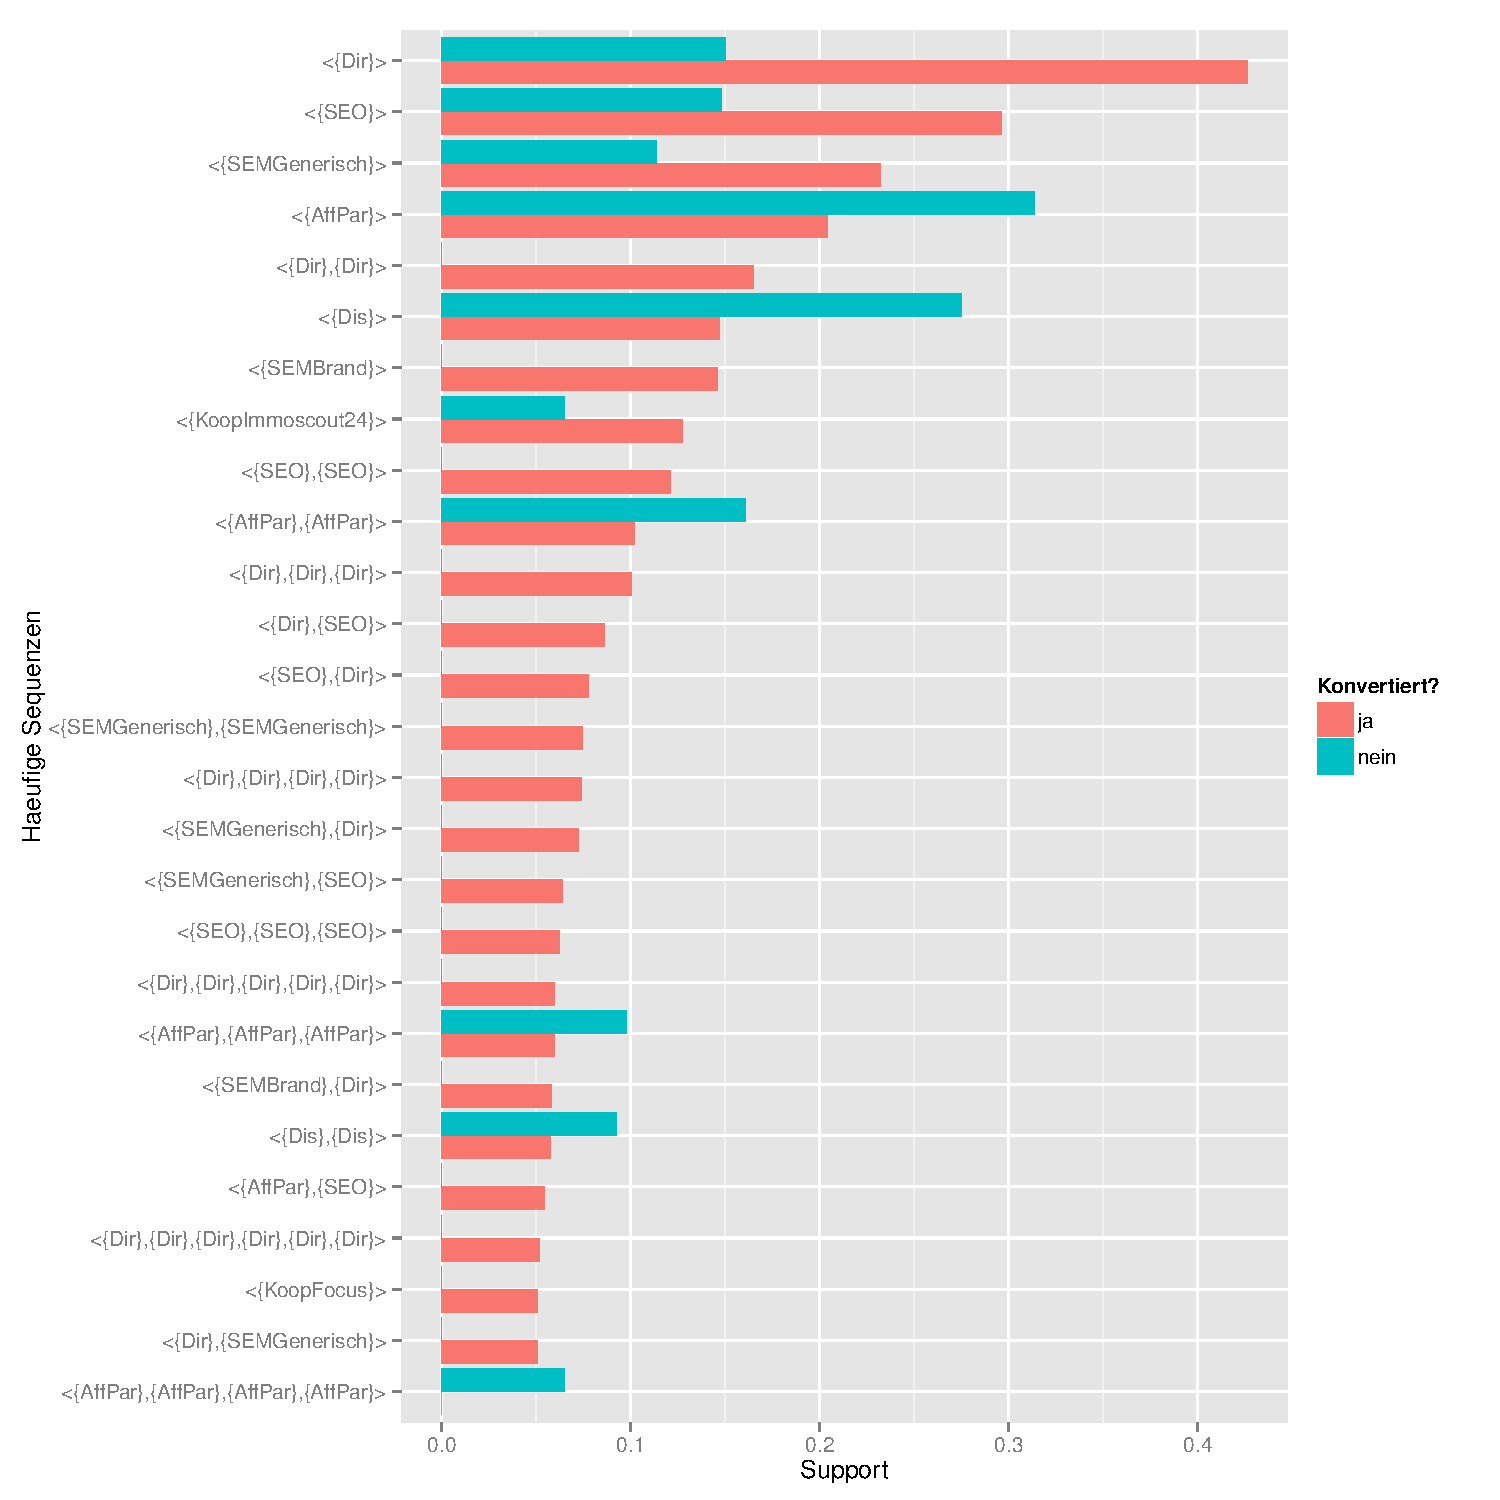
\includegraphics[scale=0.6]{spm_all.pdf}\caption[Häufige Sequenzen]{Häufige Sequenzen in den konvertierten und nicht-konvertierten Funnels}\label{spm_all}
\end{figure}
Deshalb wurde der SPADE-Algorithmus erneut seperat auf konvertierte und nicht-konvertierte Funnel angewendet, wobei dieses mal nur Funnels verwendet wurden, die eine Mindestlänge von $15$ haben. Der minimale Support wurde auf $0.2$ erhöht, um die Anzahl an häufigen Sequenzen zu beschränken. Die Ergebnisse sind in Abbildung \ref{spm_min15} dargestellt.\\
\begin{figure}[H]
	\centering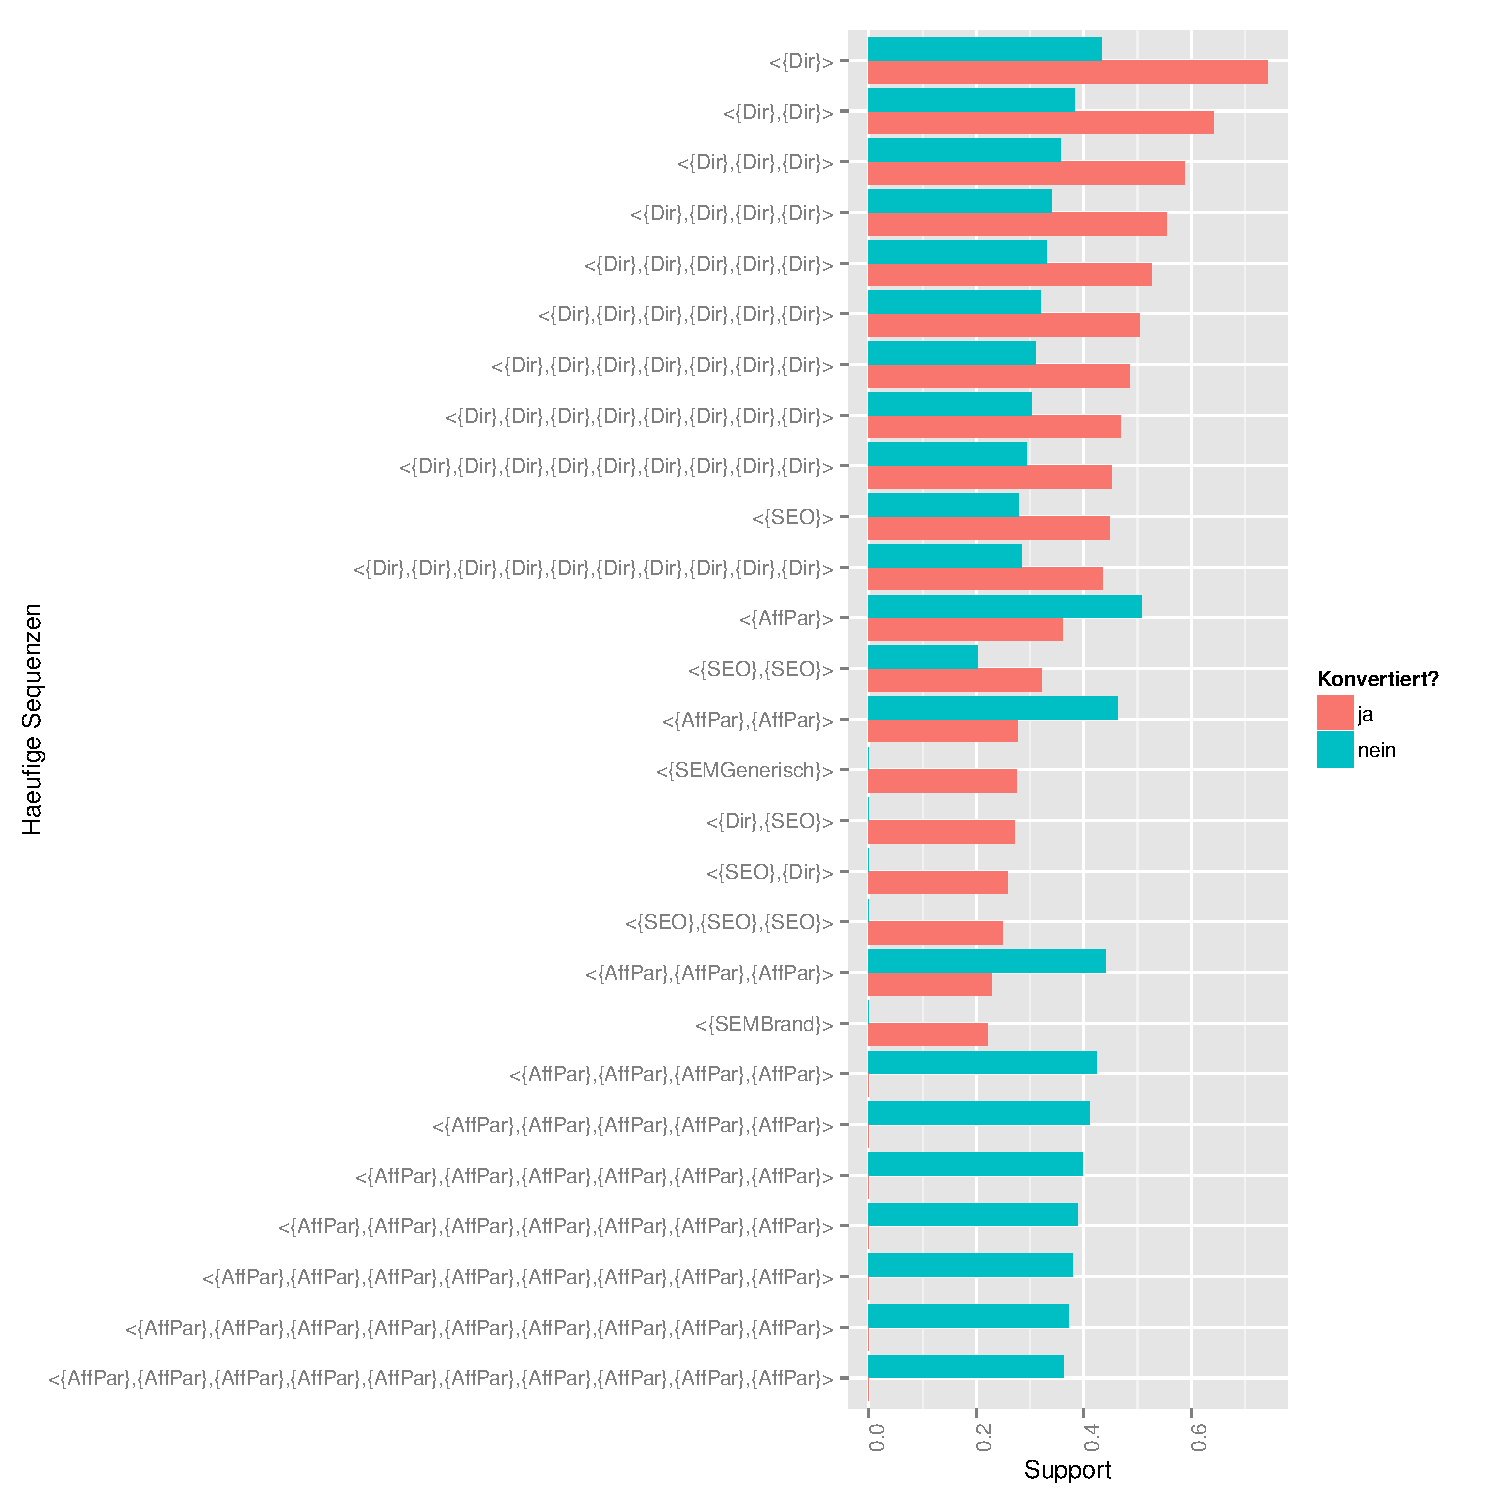
\includegraphics[scale=0.6]{spm_min15.pdf}\caption[Häufige Sequenzen in Funnels mit mindestens $15$ Kontaktpunkten]{Häufige Sequenzen in den konvertierten und nicht-konvertierten Funnels mit mindestens $15$ Kontakten}\label{spm_min15}
\end{figure}
Die Sequenzen haben jetzt teilweise einen Support, der größer als $0.5$ ist, das heißt mehr als die Hälfte der Funnels beinhalten diese Sequenz. Hier ist noch deutlicher zu erkennen, dass die \textit{Direct}-Sequenzen in den konvertierten Funnels stärker sind als in den nicht-konvertierten Funnels. Die \textit{Affiliate - Partnerprogramm}-Sequenzen haben in den nicht-konvertierten Funnels einen Support von ungefähr $40 \%$ und in den konvertierten Funnels einen Support von unter $20 \%$.\\

\subsection{Netzwerk}\label{resultsnetwork}

Mit dem Programm \textit{Gephi} ist es möglich interaktiv mit dem Netzwerk zu arbeiten. Eine komplette Analyse des Netzwerkes würde den Rahmen dieses Berichtes sprengen. Deshalb soll hier nur beispielhaft, anhand einiger Grafiken, dargestellt werden, welche Ergebnisse man aus dem Netzwerk ziehen kann. Dafür wurde ein Ausschnitt an Position $2$ gewählt. Eine genauere Anleitung zur Verwendung von \textit{Gephi} ist zudem in Kapitel \ref{anhang} zu finden.

\subsubsection*{Relative Ausgänge}

Zunächst werden die relativen Ausgänge präsentiert, das heißt die Gewichte aller Kanten, die einen Knoten verlassen, ergeben in der Summe $1$.\\
Abbildung \ref{out_labels} enthält den Ausschnitt des Netzwerkes an Position $2$ mit den relativen Ausgängen. Die Knoten sind farblich codiert und mit Labels versehen. Am rechten Bildrand ist noch eine Kampagne der ersten Position \textit{SEO\_1} zu erkennen. Von dort und den anderen Kampagnen der ersten Position führen die Kanten zu den Kampagnen der zweiten Position in der Mitte der Abbildung. Für Funnels, die mehr als zwei Kontaktpunkte haben gehen die Kanten von diesen Kampagnen zu den Knoten der dritten Positionen jenseits des linken Bildrandes. Die Kampagne \textit{Affiliate - Partnerprogramm\_3} ist noch zu erkennen.\\
Funnels, die lediglich über zwei Kontaktpunkte verfügen, enden in \textit{Fail\_2} im Falle einer Nicht-Konvertierung beziehungsweise in \textit{Success\_2} im Falle einer Konvertierung.
\begin{figure}[H]
	\centering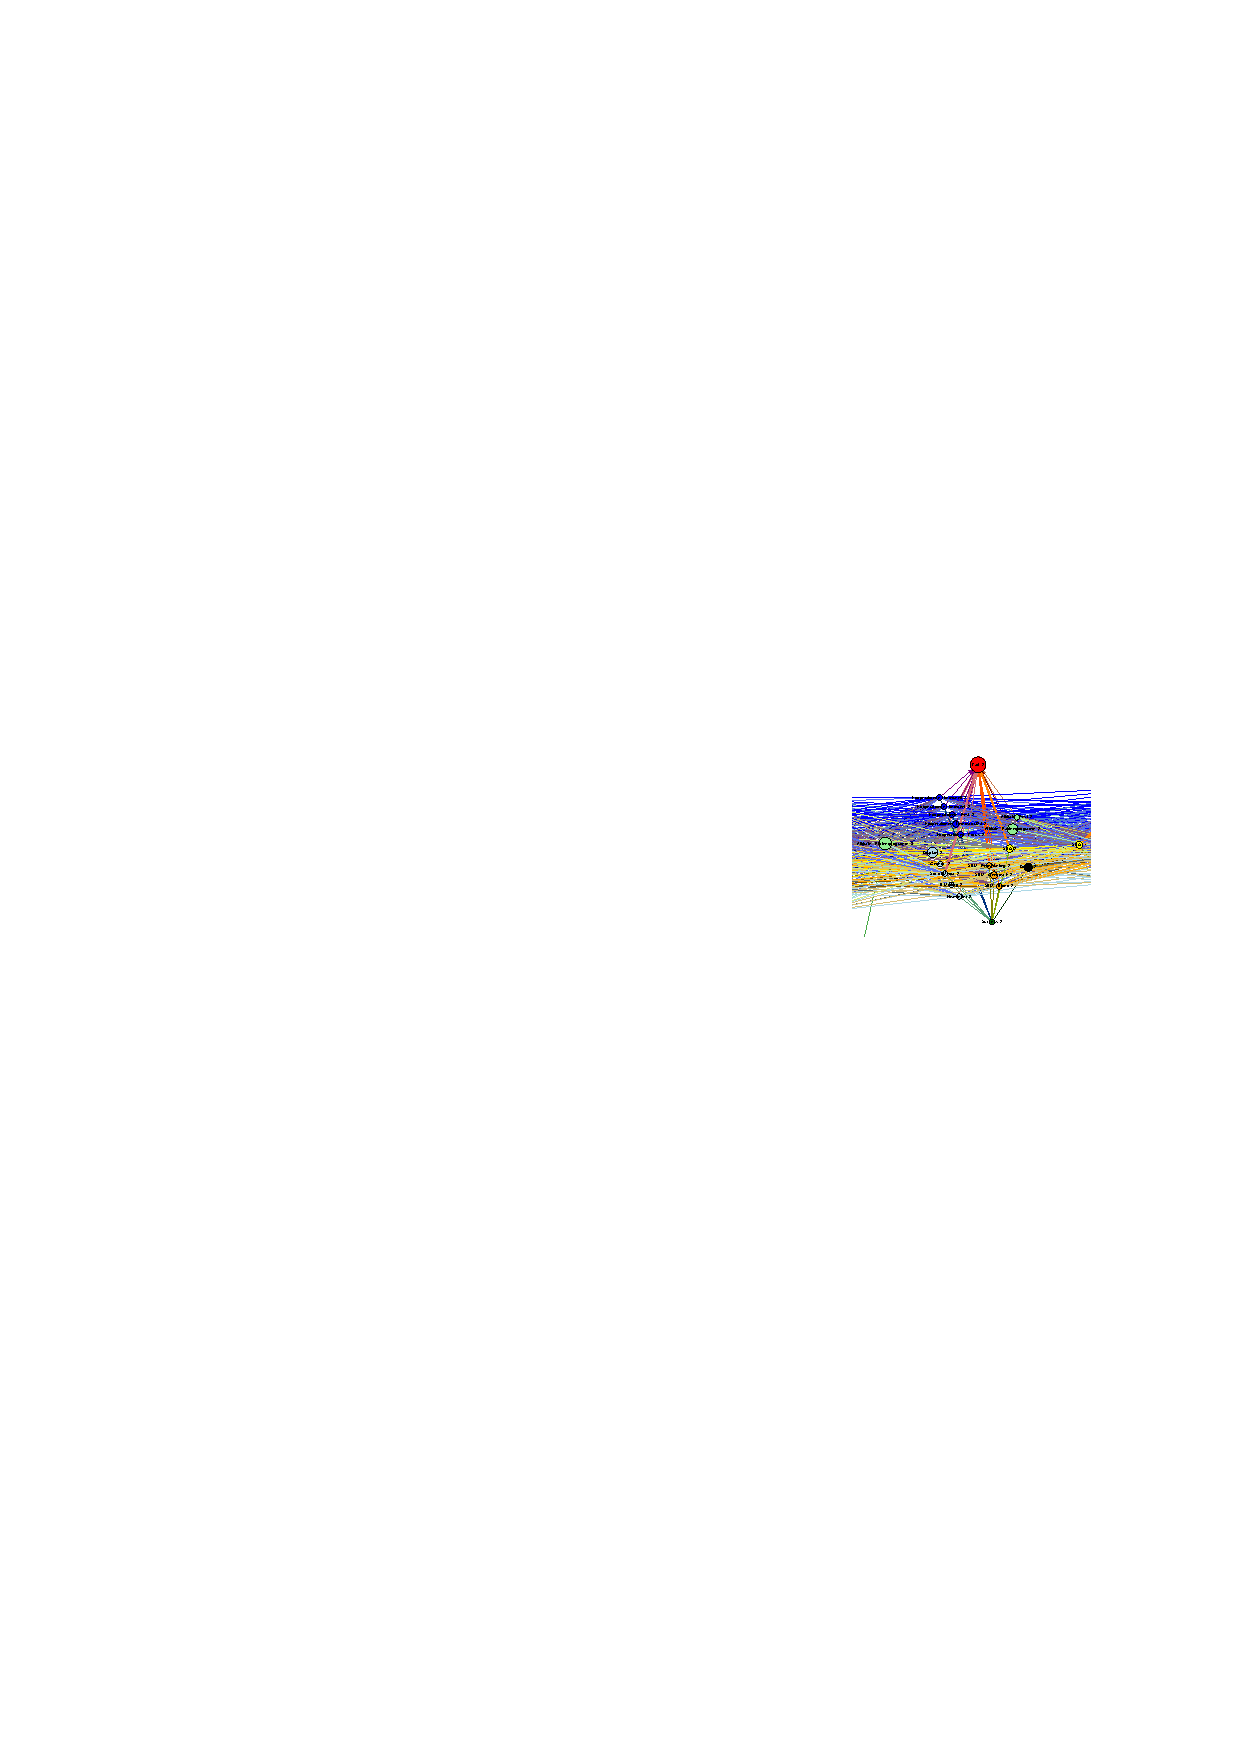
\includegraphics[scale=2.5]{out_labels.pdf}\caption[Relative Ausgänge]{Auschnitt des Netzwerkes an Position $2$ mit relativen Ausgängen}\label{out_labels}
\end{figure}
Die Dicke der Kanten hängt von deren Gewichtung ab. Abbildung \ref{out_filter_2_succ} enthält den selben Ausschnitt, wobei nun ein Filter von $0.02$ auf die Kanten angewendet wurde. Somit sind nur noch Kanten abgebildet, deren Gewicht größer als $0.02$ ist. Durch das Auswählen des Knoten \textit{Success\_2} werden alle Knoten hervorgehoben, die nach der Anwendung des Filters noch durch eine Kante mit \textit{Success\_2} verbunden sind.\\
Das heißt über $2 \%$ aller Nutzer, die als zweiten Kontaktpunkt $Direct$ haben, konvertieren an der zweiten Position. Selbiges gilt für \textit{Affiliate - Rest}, \textit{Generic}, \textit{SEM - Brand} und \textit{E-Mailing}. Durch Veränderung der Filter und weiterer Einstellungen können die Ergebnisse auch noch genauer betrachtet werden. Wie bereits erwähnt, ist in Kapitel \ref{anhang} ein Tutorial dazu vorhanden.\\
Interessant ist an dieser Stelle, dass die fünf hervorgehobenen Kampagnen gleichzeitig die fünf stärksten Kampagnen bei den Marginalen Effekten des Features \textit{Campaign} an Position $2$ sind. Das heißt die Ergebnisse des Survival-Modells können durch die Betrachtung des Netzwerkes überprüft und bestätigt werden.
\begin{figure}[H]
	\centering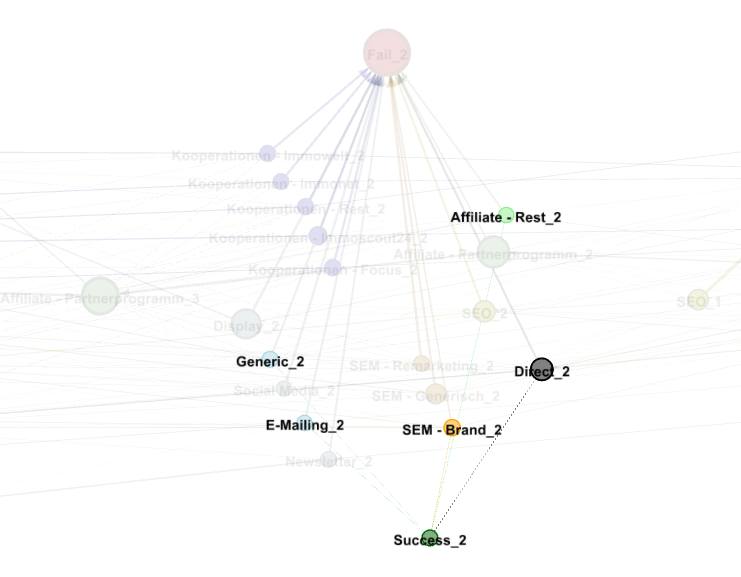
\includegraphics[scale=0.4]{out_filter_2_succ.png}\caption[Relative Ausgänge mit Filter $0.02$]{Auschnitt des Netzwerkes an Position $2$ mit relativen Ausgängen, Filter $0.02$ und Fokus auf den konvertierten Funnels}\label{out_filter_2_succ}
\end{figure}
Abbildung \ref{out_filter_50_fail} enthält erneut den selben Ausschnitt des Netzwerkes, wobei nun ein Filter von $0.5$ angewendet wurde und der Fokus auf den nicht-konvertierten Funnels liegt. Von den hervorgehobenen Knoten enden also jeweils mindestens die Hälfte der Beobachtungen ohne Konvertierung.\\
Analog zu der Betrachtung von \textit{Success\_2} oder \textit{Fail\_2} können auch die Kampagnen durch Auswählen näher betrachtet werden. Durch die positionsübergreifende Betrachtung können zudem die häufigen Sequenzen, die mittels des Sequential-Pattern-Mining Algorithmus ermittelt wurden, erkannt werden.
\begin{figure}[H]
	\centering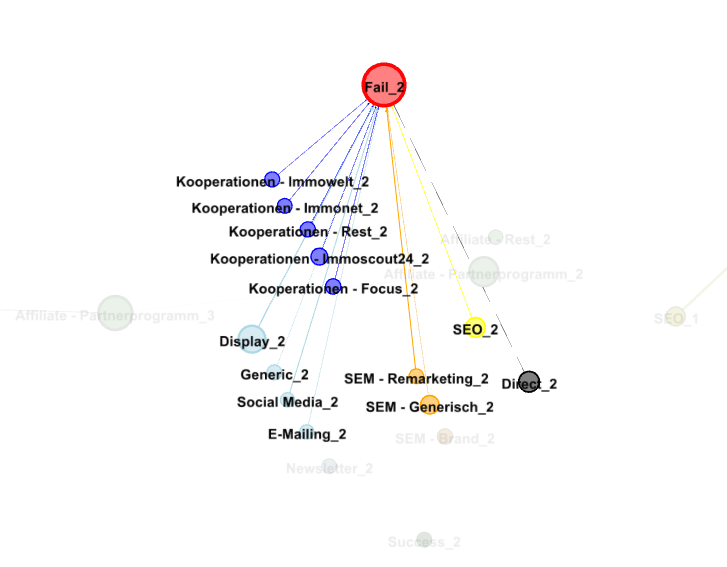
\includegraphics[scale=0.4]{out_filter_50_fail.png}\caption[Relative Ausgänge mit Filter $0.5$]{Auschnitt des Netzwerkes an Position $2$ mit relativen Ausgängen, Filter $0.5$ und Fokus auf den nicht-konvertierten Funnels}\label{out_filter_50_fail}
\end{figure}

\subsubsection*{Relative Eingänge}

In diesem Abschnitt wird erneut Position $2$ betrachtet, wobei die Kanten nun anhand der relativen Eingänge gewichtet sind. Das heißt die Gewichte aller Kanten, die in einen bestimmten Knoten gehen, ergeben aufsummiert $1$. Abbildung \ref{in_labels} enthält den Ausschnitt des Netzwerkes. Am rechten beziehungsweise linken Bildrand ist erneut eine Kampagne von Position $1$ beziehungsweise $3$ zu erkennen. Die Farben und Beschriftungen der Knoten sind die selben wie in Abbildung \ref{out_labels}. 
\begin{figure}[H]
	\centering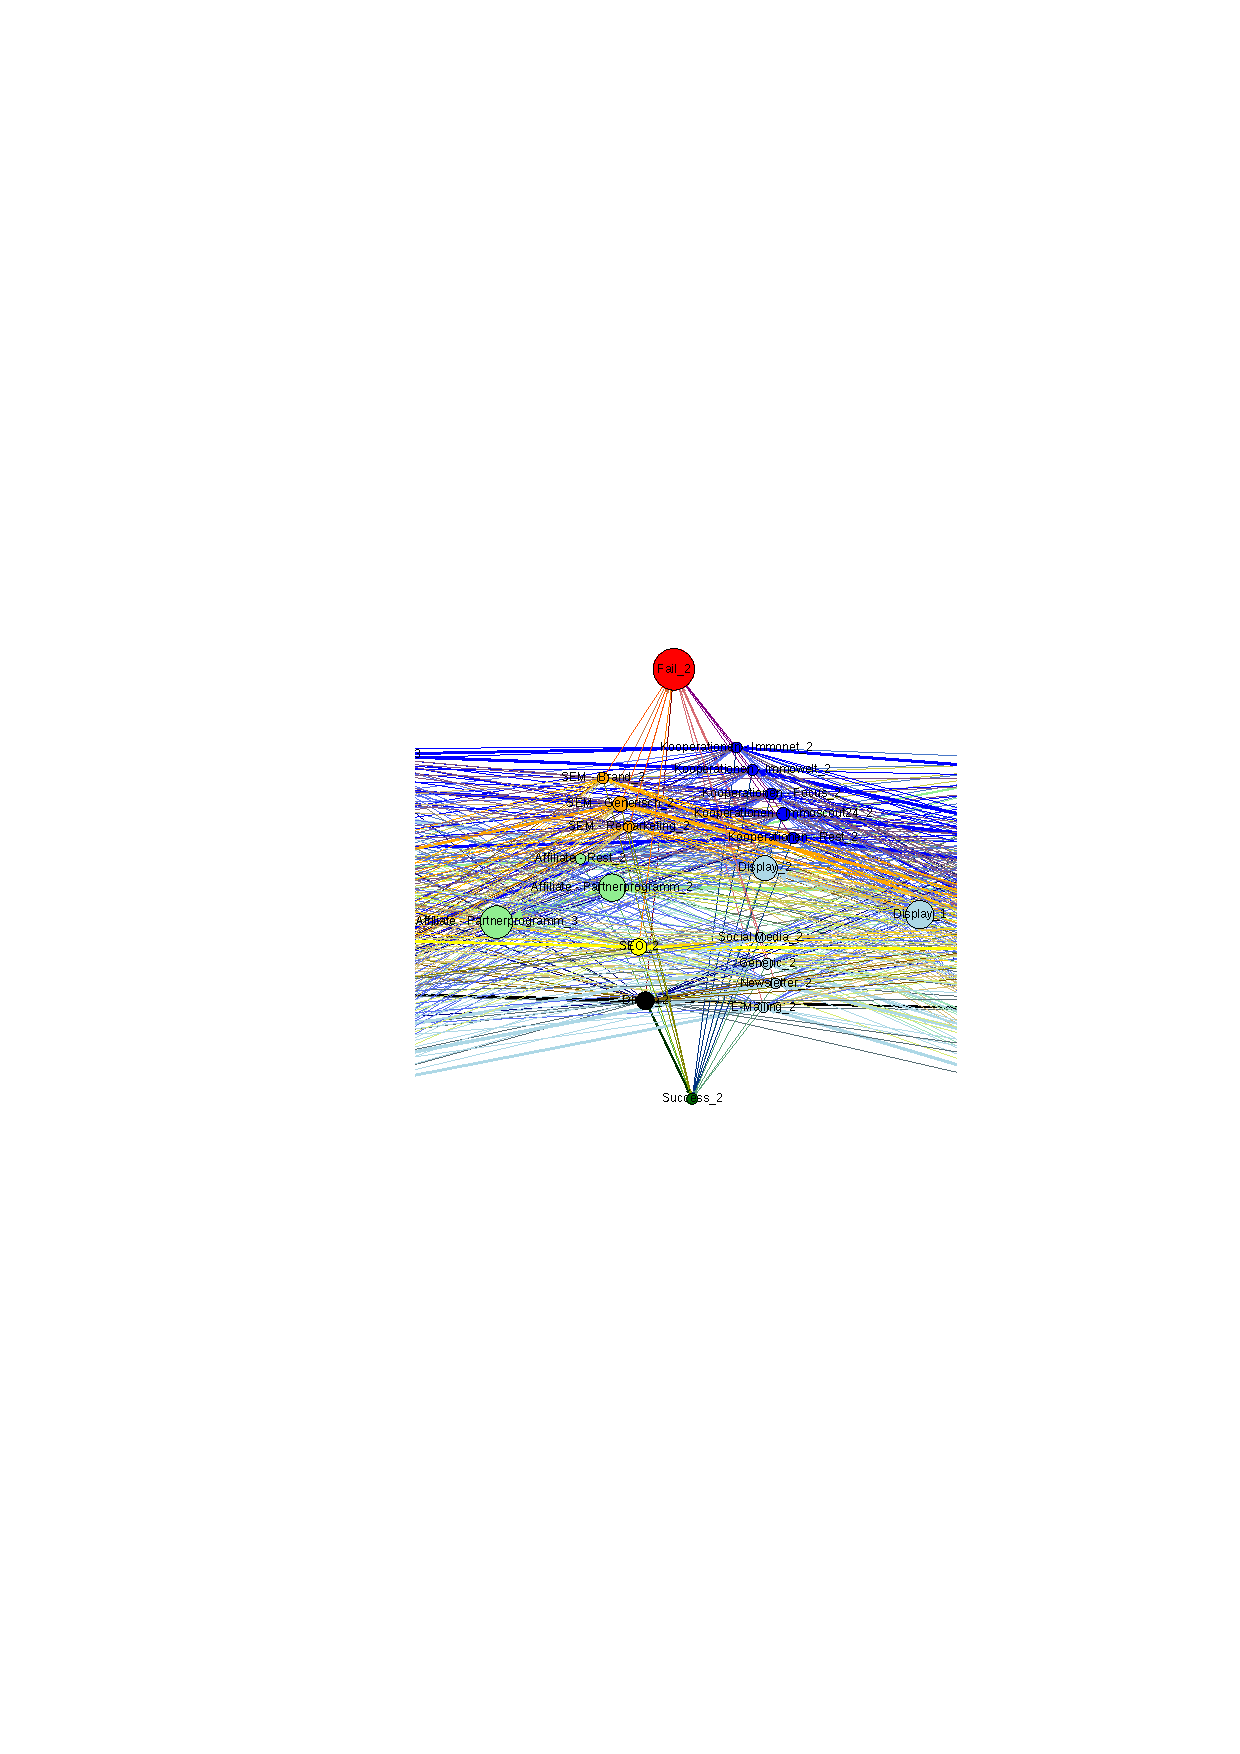
\includegraphics[scale=1]{in_labels.pdf}\caption[Relative Eingänge]{Auschnitt des Netzwerkes an Position $2$ mit relativen Eingängen}\label{in_labels}
\end{figure}
Auf diesen Ausschnitt wurde ein Filter von $0.1$ angewendet, wobei der Fokus auf den konvertierten Funnels liegt (siehe Abbildung \ref{in_filter_10_succ}). Die hervorgehobenen Knoten \textit{SEM-Generisch\_2}, \textit{Display\_2}, \textit{SEO\_2} und \textit{Direct\_2} machen jeweils mehr als $10 \%$ der konvertierten Funnels aus, die aus zwei Kontaktpunkten bestehen. Das heißt hier kann nun betrachtet werden, aus welchen Kampagnen des letzten Kontaktpunktes sich die Menge der konvertierten beziehungsweise nicht-konvertierten Funnels zusammensetzen. Zudem ist es auch möglich eine Kampagne zu markieren, so dass erkennbar wird, aus welchen Kampagnen der vorherigen Position, sich diese zusammensetzt. Im Gegensatz dazu, war die Interpretation im vorherigen Kapitel eine andere. Dort wurde betrachtet, wohin die Nutzer von einem Knoten aus gehen.
\begin{figure}[H]
	\centering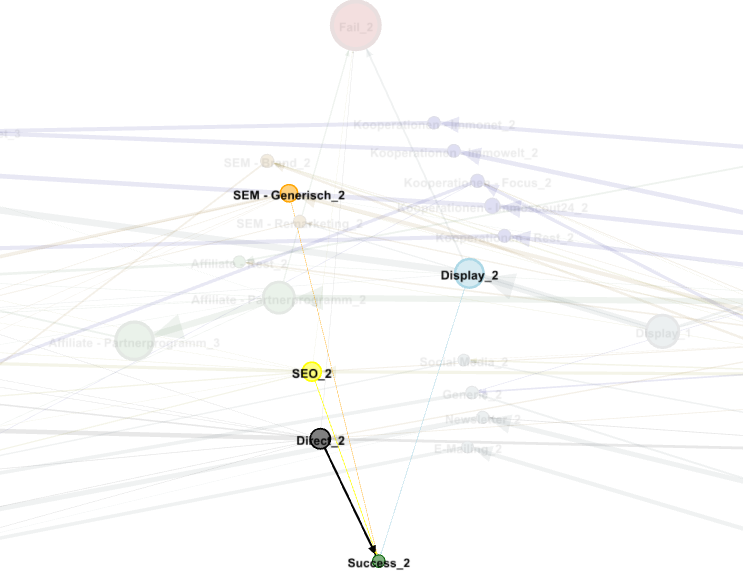
\includegraphics[scale=0.4]{in_filter_10_succ.png}\caption[Relative Eingänge mit Filter $0.1$ und Fokus auf Konvertierten]{Auschnitt des Netzwerkes an Position $2$ mit relativen Eingängen, Filter $0.1$ und Fokus auf den konvertierten Funnels}\label{in_filter_10_succ}
\end{figure}
Abbildung \ref{in_filter_10_fail} enthält den selben Ausschnitt mit dem selben Filter von $0.1$, wobei nun die nicht-konvertierten Funnels betrachtet werden. Das heißt von den Funnels, die nach zwei Kontaktpunkten ohne Konvertierung abbrechen, haben jeweils mindestens $10\%$ als letzten Kontaktpunkt \textit{Affiliate - Partnerprogramm\_2}, \textit{Display\_2}, \textit{SEO\_2} oder \textit{Direct\_2}.
\begin{figure}[H]
	\centering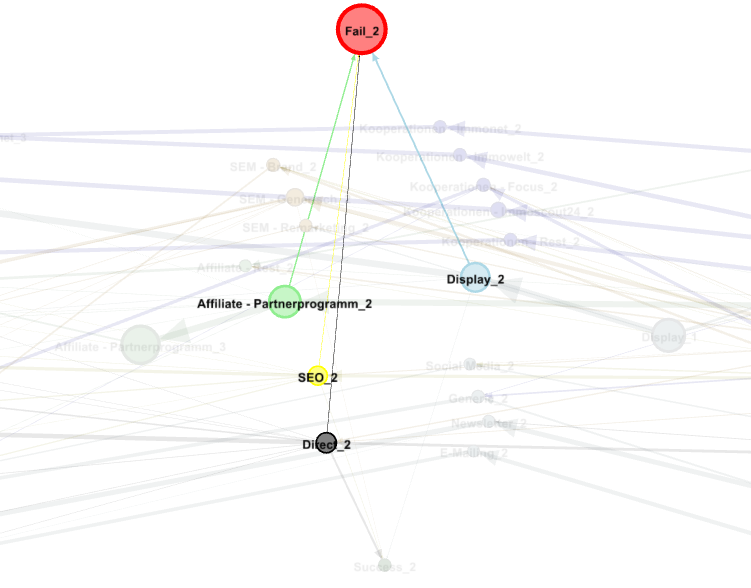
\includegraphics[scale=0.4]{in_filter_10_fail.png}\caption[Relative Eingänge mit Filter $0.1$ und Fokus auf Nicht-Konvertierten]{Auschnitt des Netzwerkes an Position $2$ mit relativen Eingängen, Filter $0.1$ und Fokus auf den nicht-konvertierten Funnels}\label{in_filter_10_fail}
\end{figure}
\section{Zusammenfassung}

\begin{frame}\frametitle{Inhalt}
	\tableofcontents[currentsection,hideallsubsections]
\end{frame}

\begin{frame}\frametitle{Zusammenfassung der Ergebnisse}
	\begin{itemize}
		\item Zeitdiskretes Survival-Modell
		\begin{itemize}
			\item Klassifikation in konvertierte und nicht-konvertierte Funnels
			\item Marginale Effekte der Features
		\end{itemize}
		\item Sequential Pattern Mining
		\item Netzwerk
		\begin{itemize}
			\item Visualisierung der gesamten Daten
			\item Bestätigung der Ergebnisse aus Survival-Modell und Sequential Pattern Mining
			\item Tutorial zum interaktiven Arbeiten im Bericht
		\end{itemize}
	\end{itemize}
\end{frame}

\begin{frame}{Literatur}
	\begin{thebibliography}{1}
		\bibitem{} J. H. Friedman \& B. E. Popescu (2005): {\glqq Predictive Learning via Rule Ensembles\grqq}.
		\bibitem{} R. Agrawal \& R. Srikant (1995): {\glqq Mining sequential patterns\grqq}.
		\bibitem{} M. J. Zaki (2001): {\glqq SPADE: An efficient algorithm for mining frequent sequences\grqq}.
		\bibitem{} M. Bastian, S. Heymann \& M. Jacomy. (2009): {\glqq Gephi: An Open Source Software for Exploring and Manipulating Networks\grqq}.
		\bibitem{} R-Packages: \textit{gbm, rgexf, arulesSequences, data.table, plyr, ggplot2, doSNOW, foreach}.
	\end{thebibliography}
\end{frame} 

\begin{frame}
	\centering \huge
	Vielen Dank für Ihre Aufmerksamkeit!
\end{frame}

\end{document}

